% Estas slides tienen que abrirse con el programa pdfpc que soporta videos embebidos
% el comando es: pdfpc -g slides.pdf
% para los videos se requiere ubuntu-restricted-extras
% para la bibliografía se requiere biber y configurar texstudio

%\documentclass[compress,handout]{beamer}
\documentclass[aspectratio=169,compress]{beamer}

% add beamer preamble
% Theme customization
\setbeamertemplate{itemize item}[rectangle] % configure itemize
\setbeamertemplate{itemize subitem}[circle] % configure itemize
\setbeamertemplate{itemize subsubitem}[triangle] % configure itemize
\setbeamertemplate{navigation symbols}{} % remover simbolos de navegacion de las slides
\usefonttheme[onlymath]{serif} % simbolos matematicos en serif (Como es en latex original)
\setbeamersize{text margin left=3mm,text margin right=3mm} 

\setbeamertemplate{blocks}[rounded] % blocks corners rounded
\setbeamercolor{block body}{bg=blue!12,fg=black} % color of blocks
\setbeamertemplate{caption}{\raggedright\insertcaption\par} % elimina la palabra "Figura" del caption

\usepackage[overridenote]{pdfpc} % requires to download manually pdfpc.sty package from https://www.ctan.org/pkg/pdfpc

% add latex preamble
% para la bibliografía se requiere biber y configurar texstudio

% Latex packages
\usepackage[utf8]{inputenc}
\usepackage[T1]{fontenc} % para copiar acentos en español del pdf y permite acentos en las notas
\usepackage[spanish]{babel}
\usepackage[per-mode = symbol]{siunitx} % para manejar las unidades
\usepackage{multimedia} % to add videos with \movie command
\usepackage{multirow}
\usepackage{graphicx}
\usepackage{xcolor}
\usepackage{amsmath} % bmatrix
\usepackage[makeroom]{cancel} % \cancel to cancel terms in math equations
\renewcommand{\CancelColor}{\color{red}} % set red color for \cancel command
\usepackage[caption=false]{subfig} % caption = false elimina la palabra "Figura" del caption
\usepackage{import} % para el comando import (se usa para pdf_tex)
\captionsetup[subfigure]{labelformat=empty} % remover el indice del caption de la subfigura
\usepackage{booktabs} % \toprule \midrule \bottomrule
\usepackage[backend=biber]{biblatex} % set biber to format references. Must configure Biber in Texstudio
\usepackage{csquotes} % to remove warning triggered by biblatex and babel
\usepackage{algorithm} % to put captions to the algorithmics environmets
\usepackage{algpseudocode} % to write algorithm
\usepackage{tikz} % to use tikz
\usetikzlibrary{fit} % to fit a node around other nodes in tikz
\usepackage[export]{adjustbox} % valign in subfloat
\usepackage{colortbl} % to paint cells in a table

% Color commands for annotations
\newcommand\TODO[1]{\textbf{\textcolor{red}{#1}}} %  TODO notes

% Graphic paths
\graphicspath{{./images/}}

% listings configuration for C code
\usepackage{listings} % code
\definecolor{commentgreen}{RGB}{2,112,10}
\definecolor{eminence}{RGB}{108,48,130}
\definecolor{weborange}{RGB}{255,165,0}
\definecolor{frenchplum}{RGB}{129,20,83}

\lstset{ % spanish characters for listings package
	inputencoding=latin1,
    columns=fullflexible,
	breaklines=true,
	tabsize=2,
	showstringspaces=false,
	basicstyle=\ttfamily,
	backgroundcolor=\color{lightgray}, % Choose background color
	literate={á}{{\'a}}1
	{ã}{{\~a}}1
	{é}{{\'e}}1
	{ó}{{\'o}}1
	{í}{{\'i}}1
	{ñ}{{\~n}}1
	{¡}{{!`}}1
	{¿}{{?`}}1
	{ú}{{\'u}}1
	{Í}{{\'I}}1
	{Ó}{{\'O}}1
    {-}{-}1
}

\lstdefinestyle{cpp}{ % spanish characters for listings package
    language=C++,
   	commentstyle=\color{commentgreen},
    keywordstyle=\color{eminence},
    stringstyle=\color{red},
    emph={int,char,double,float,unsigned,void,bool},
    emphstyle={\color{blue}}
}

\lstdefinestyle{bash}{ % spanish characters for listings package
	language=Bash
}

\lstdefinestyle{xml}{
	language=XML,
	morekeywords={encoding,xs:schema,xs:element,xs:complexType,xs:sequence,xs:attribute}
}

\lstdefinestyle{cmake}{
	language=make, % there is no cmake support in listings
}

\lstdefinestyle{python}{
    language=python,
}


%%%%% PARA QUE EN LAS TABLAS SE PUEDA PONER UN SALTO DE LINEA DENTRO DE UNA CELDA
\newcommand{\specialcell}[2][c]{%
    \begin{tiny}
        \begin{tabular}[#1]{@{}c@{}}#2\end{tabular}  
    \end{tiny}
}
%%%%%%%%%%%%%%%%%%%%%%%%%%%%%%%%%%%%%%%%%%%%%%%%%%%%%%%%%%%%%%%%%%%%%%%%

%%%%% PARA QUE LAS TABLAS TENGAN TODAS LAS COLUMNAS CENTRADAS Y DE IGUAL TAMAÑO
\usepackage{tabularx}
\renewcommand{\tabularxcolumn}[1]{>{\centering\arraybackslash}m{#1}}
%%%%%%%%%%%%%%%%%%%%%%%%%%%%%%%%%%%%%%%%%%%%%%%%%%%%%%%%%%%%%%%%%%%%%%%%



% add math preamble
\usepackage{amsmath}
\usepackage{amssymb}
\usepackage{amsopn}
\usepackage{mathtools}

% math
\renewcommand{\vec}[1]{\boldsymbol{\mathbf{#1}}}
\newcommand{\norm}[1]{\lVert#1\rVert}

% Declare arg max and arg min functionss
\DeclareMathOperator*{\argmax}{arg\,max}
\DeclareMathOperator*{\argmin}{arg\,min}

% Homogeneous decoration function
\newcommand{\homo}[1]{\dot{#1}}


% Declare projection as math function
\DeclareMathOperator{\proj}{proj}
\newcommand{\fromCoord}[2]{{#1}_\mathrm{#2}}
\newcommand{\toCoord}[2]{\prescript{\mathrm{#2}}{}{#1}}
\newcommand{\worldCoordSystem}{\mathrm{w}}
\newcommand{\bodyCoordSystem}{\mathrm{B}}
\newcommand{\cameraCoordSystem}{\mathrm{c}}
\newcommand{\point}{\vec{p}}
\newcommand{\worldPoint}{\toCoord{\point}{\worldCoordSystem}}
\newcommand{\imagePoint}{\vec{u}}
\newcommand{\cameraPoint}{\toCoord{\point}{\cameraCoordSystem}}
\newcommand{\homoWorldPoint}{\toCoord{\homo{\point}}{\worldCoordSystem}}
\newcommand{\homoImagePoint}{\homo{\imagePoint}}
\newcommand{\homoCameraPoint}{\toCoord{\homo{\point}}{\cameraCoordSystem}}
\newcommand{\measurement}{\vec{z}}
\newcommand{\prediction}{\hat{\vec{z}}}
\newcommand{\seMatrix}{\vec{\xi}}
\newcommand{\transform}[2]{\toCoord{\fromCoord{\seMatrix}{#2}}{#1}}
\newcommand{\pointCoord}[1]{\toCoord{\point}{#1}}
\newcommand{\rotation}{\vec{R}}
\newcommand{\rotationCoord}[2]{\toCoord{\fromCoord{\rotation}{#2}}{#1}}
\newcommand{\translation}{\vec{t}}
\newcommand{\translationCoord}[2]{\toCoord{\fromCoord{\translation}{#2}}{#1}}
\newcommand{\intrinsicMatrix}{\vec{K}}
\newcommand{\principalPoint}{\vec{c}}
\newcommand{\reprojectionError}{u}
\newcommand{\projectionMatrix}{\vec{P}}
\newcommand{\cameraCenter}{\vec{o}}
\newcommand{\essentialMatrix}{\vec{E}}
\newcommand{\inverse}[1]{{#1}^{-1}}

% Motion model
\newcommand{\position}{\vec{p}}
\newcommand{\orientationQuaternion}{\vec{q}}
\newcommand{\predictedPosition}{\hat{\vec{p}}}
\newcommand{\predictedOrientationQuaternion}{\hat{\vec{q}}}
\newcommand{\linearVelocity}{\vec{v}}
\newcommand{\angularVelocity}{\vec{\omega}}

\DeclareMathOperator{\slerpOp}{slerp}
\newcommand{\slerp}[1]{\slerpOp{\left( #1 \right)}}

% Map structure
\newcommand{\map}{M}
\newcommand{\keyframesSet}{K}
\newcommand{\mapPointsSet}{P}
\newcommand{\observedMapPoints}{O}
\newcommand{\covisibilityKeyframes}{CK}
\newcommand{\localMap}{local\_map}



% Bundle Adjutment
\newcommand{\update}{\vec{\delta}}
\newcommand{\incremental}{\hat{\update}}


% Loop Closure names

% scaled operators and letters to fancy view
\newcommand{\sminus}{\scalebox{0.5}[1.0]{$-$}}
\newcommand{\splus}{\scalebox{0.6}[0.6]{$+$}}
\newcommand{\curr}{c}
\newcommand{\sind}[1]{\scalebox{0.6}[0.6]{$#1$}}
\newcommand{\ind}[1]{\scalebox{0.7}[0.7]{$#1$}}

\newcommand{\keyframe}{\vec{K}}
\newcommand{\bowVector}{\vec{v}}
\newcommand{\lcError}{\vec{\Omega}}
\newcommand{\relativeTransformation}{\seMatrix}
\DeclareMathOperator{\interpolate}{interpolate}

\newcommand{\relativeMotion}{\vec{\delta}}
\newcommand{\groundTruth}[1]{{#1}^{*}}



% definición del operador rot()
\DeclareMathOperator{\rotationOp}{rot}
\newcommand{\getRotation}[1]{\rotationOp{\left( #1 \right)}}

\DeclareMathOperator{\translationOp}{trans}
\newcommand{\getTranslation}[1]{\translationOp{\left( #1 \right)}}









\title{Sensores}
\author{}
\institute{Universidad Nacional de Rosario}
%\date{\scriptsize{Julio 1, 2021}}
\date{}

\begin{document}

% add title page
\frame{\titlepage}

\section{Sensores}
\begin{frame}
    \frametitle{Tipos de sensores}

    \begin{itemize}
    \item sensores propioceptivos miden valores internos del sistema (robot), por ejemplo, velocidad del motor, carga de la rueda, ángulos de articulación del brazo del robot y voltaje de la batería.

    \item sensores exteroceptivos adquieren información del entorno del robot, por ejemplo, medidas de distancia, intensidad de la luz y amplitud del sonido. Por lo tanto, el robot interpreta las mediciones de los sensores exteroceptivos para extraer características ambientales significativas.
    \end{itemize}

    \begin{itemize}
    \item Los sensores pasivos miden la energía ambiental que ingresa al sensor. Los ejemplos de sensores pasivos incluyen sondas de temperatura, micrófonos y cámaras CCD o CMOS.

    \item Los sensores activos emiten energía al medio ambiente y luego miden la reacción ambiental. Debido a que los sensores activos pueden gestionar interacciones más controladas con el medio ambiente, a menudo logran un rendimiento superior. Sin embargo, la detección activa presenta varios riesgos: la energía de salida puede afectar las mismas características que el sensor está intentando medir. Además, un sensor activo puede sufrir interferencias entre su señal y las que están fuera de su control. Por ejemplo, las señales emitidas por otros robots cercanos, o sensores similares en el mismo robot, pueden influir en las mediciones resultantes. Los ejemplos de sensores activos incluyen codificadores de cuadratura de rueda, sensores ultrasónicos y telémetros láser.
\end{itemize}


\end{frame}


\begin{frame}
    \frametitle{Sensores}
    \TODO{poner tabla 4.1 del libro siegwart}

\end{frame}



\begin{frame}
    \frametitle{Optical encoders}
    \scriptsize
    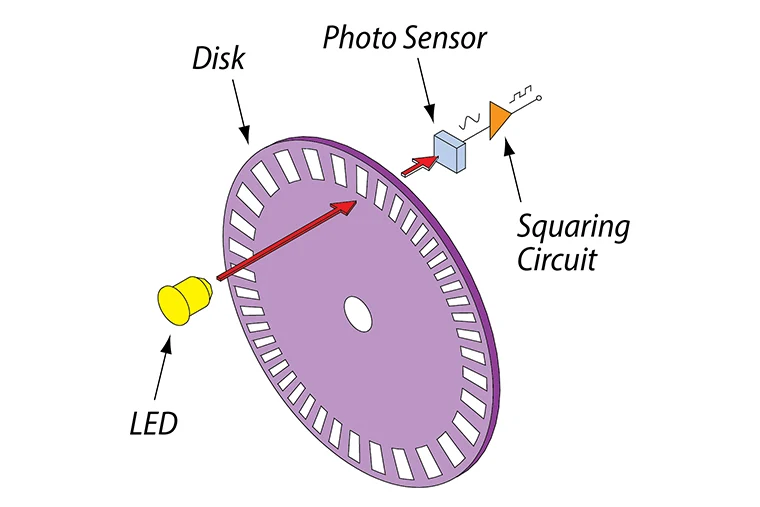
\includegraphics[width=0.45\columnwidth]{images/encoder_principle}
    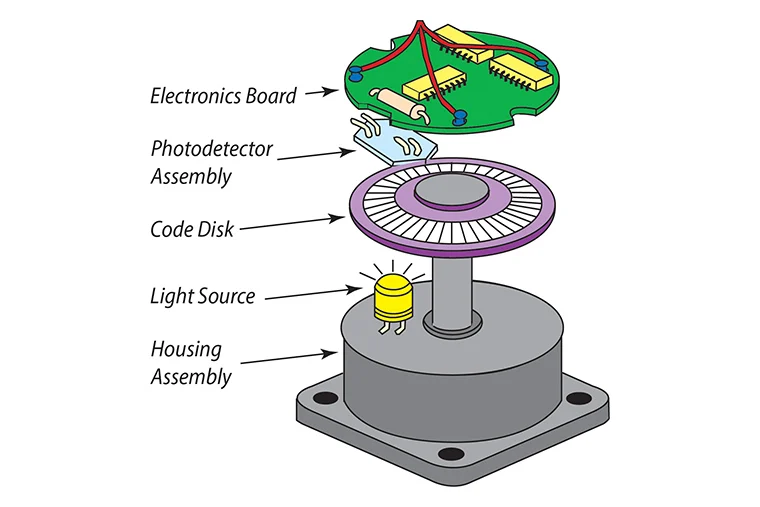
\includegraphics[width=0.46\columnwidth]{images/encoder_parts}
    \footnotesize

    \begin{block}{Principio de funcionamiento}
        Consta de una fuente de iluminación, una rejilla fija que enmascara la luz, un disco rotor con una fina rejilla óptica que gira con el eje y detectores ópticos fijos. A medida que el rotor se mueve, la cantidad de luz que incide en los detectores ópticos varía según la alineación de las rejillas fijas y móviles. En robótica, la onda sinusoidal resultante se transforma en una onda cuadrada discreta utilizando un umbral para elegir entre estados claros y oscuros. La resolución se mide en ciclos por revolución (CPR). La resolución angular mínima se puede calcular fácilmente a partir de la clasificación de CPR de un codificador. Un codificador típico en robótica móvil puede tener 2000 CPR
    \end{block}
\end{frame}

\begin{frame}
    \frametitle{Optical encoders}

    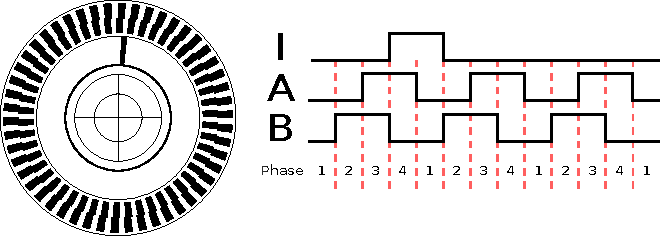
\includegraphics[width=\columnwidth]{images/encoder.pdf}
    \footnotesize

    La relación de fase observada entre los trenes de impulsos del canal A y B se utiliza para determinar la dirección de rotación. Una sola ranura en la pista interior genera un pulso de referencia (índice) por revolución.

    \begin{itemize}
        \item Proprioceptivo
        \item La resolución se mide en ciclos por revolución (CPR). Suelen tener 2000 CPR.
        \item La odometría basada en encoders acumula error rápidamente por diferencias físicas en en las ruedas, deslizamiento o giro en el aire de las ruedas.
    \end{itemize}
\end{frame}

\begin{frame}
    \frametitle{Bumper}

\end{frame}


\begin{frame}
    \frametitle{Compass}

        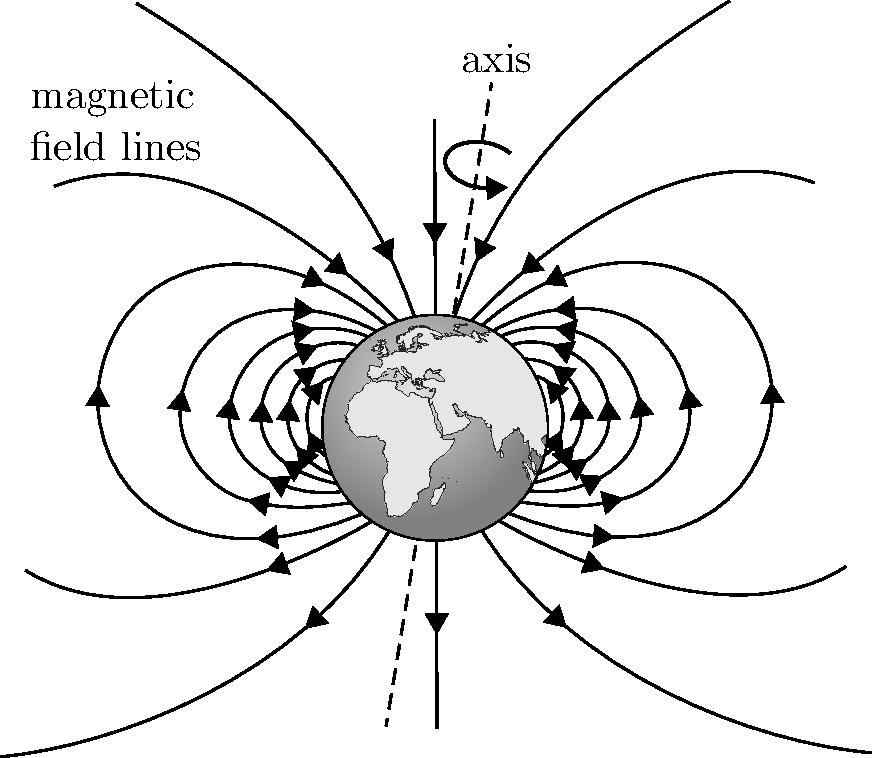
\includegraphics[width=0.4\columnwidth]{images/earth_magnetic_field.pdf}
        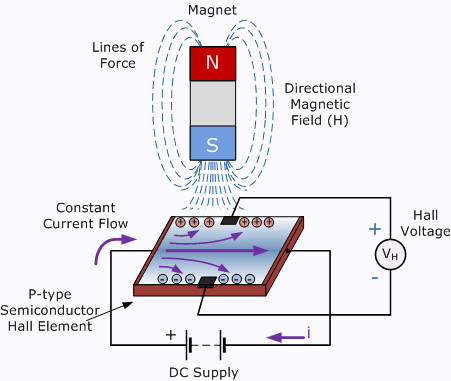
\includegraphics[width=0.4\columnwidth]{electromagnetism.jpg}

    \begin{block}{Principio de funcionamiento}

    \end{block}
\end{frame}

\begin{frame}
    \frametitle{Compass}

    \begin{center}
        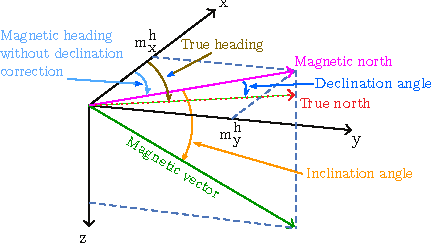
\includegraphics[width=0.5\columnwidth]{images/magnetic_field.pdf}
    \end{center}

    \begin{itemize}
        \item exteroceptivo
        \item
    \end{itemize}
\end{frame}

\begin{frame}
    \frametitle{Compass}

    \begin{center}
        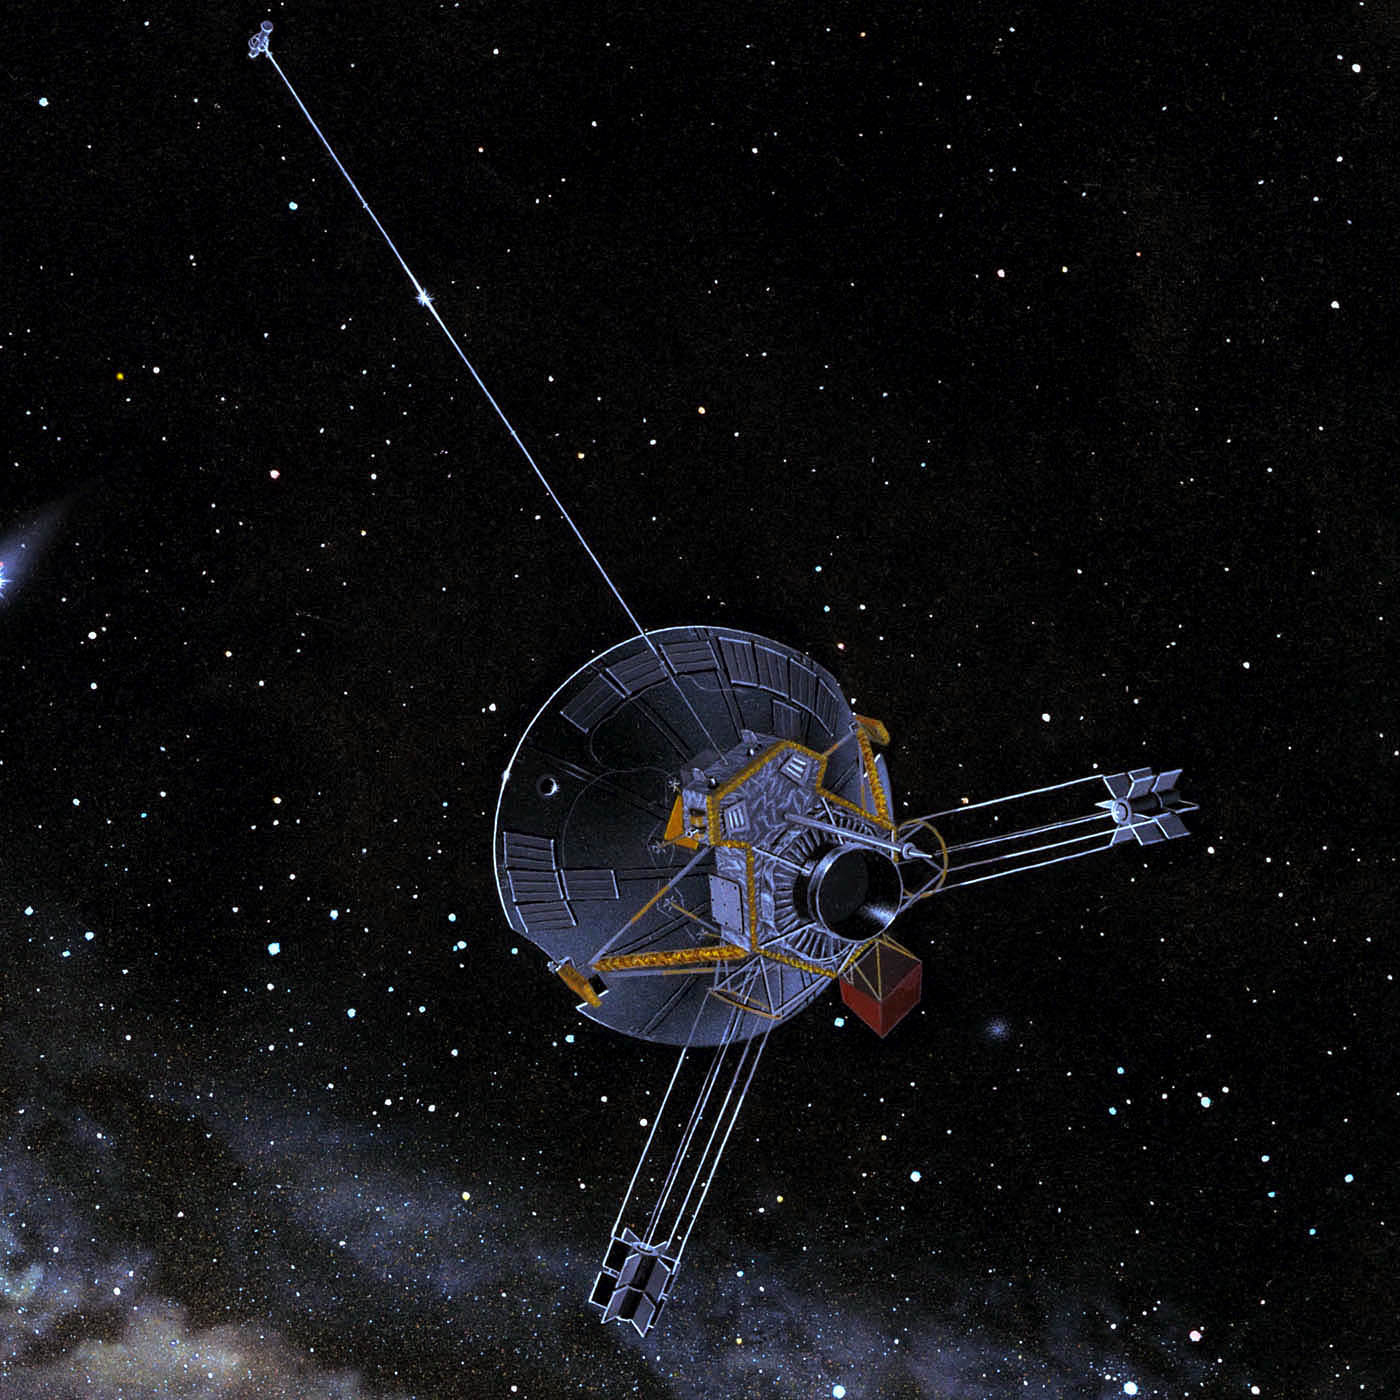
\includegraphics[width=0.5\columnwidth]{pioneer_10.jpg}
    \end{center}
\end{frame}

\begin{frame}
    \frametitle{Giróscopo o Giroscopio}
    \scriptsize
    \begin{center}
        \movie[autostart,loop,poster]{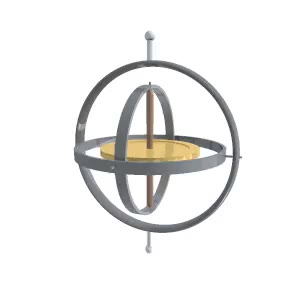
\includegraphics[width=0.25\columnwidth]{./images/gyroscope_video.jpg}}{./videos/gyroscope.mp4}
        \hspace{1em}
        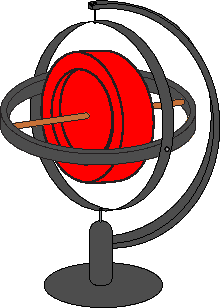
\includegraphics[width=0.15\columnwidth]{images/gyroscope.pdf}
        \hspace{1em}
        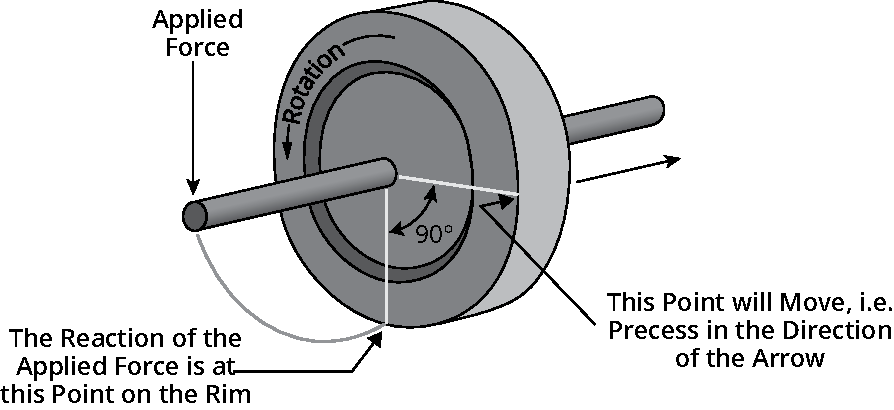
\includegraphics[width=0.4\columnwidth]{images/gyroscope_precession.pdf}
    \end{center}

    \begin{block}{Principio de funcionamiento}
        \begin{itemize}
            \item Un giróscopo es todo cuerpo simétrico en rotación a una velocidad suficiente como para experimentar los efectos giroscópicos.
            \item Los giróscopos son dispositivos que miden o mantienen el movimiento de rotación.
        \end{itemize}

    \end{block}

    \begin{itemize}
        \item Introceptivo
        \item Pasivo
        \item Mide Velocidad Angular
        \item Unidad de medición $\si{\degree\per\second}$ o Revoluciones por Minuto (RPM)
    \end{itemize}

    \note{https://answeringatpl.com/instrumentation/gyroscopic-principles/\\
          https://www.5hertz.com/index.php?route=tutoriales/tutorial&tutorial_id=13
      }

\end{frame}

\begin{frame}
    \frametitle{Giróscopo: Principios giroscópicos}
    \note{https://www.youtube.com/watch?v=nhNg-8RSuKY}
    \scriptsize
    
    \begin{center}
        \movie[autostart,loop,poster]{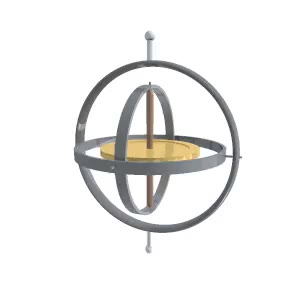
\includegraphics[width=0.25\columnwidth]{./images/gyroscope_video.jpg}}{./videos/gyroscope.mp4}
        \hspace{1em}
        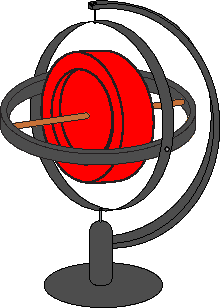
\includegraphics[width=0.15\columnwidth]{images/gyroscope.pdf}
        \hspace{1em}
        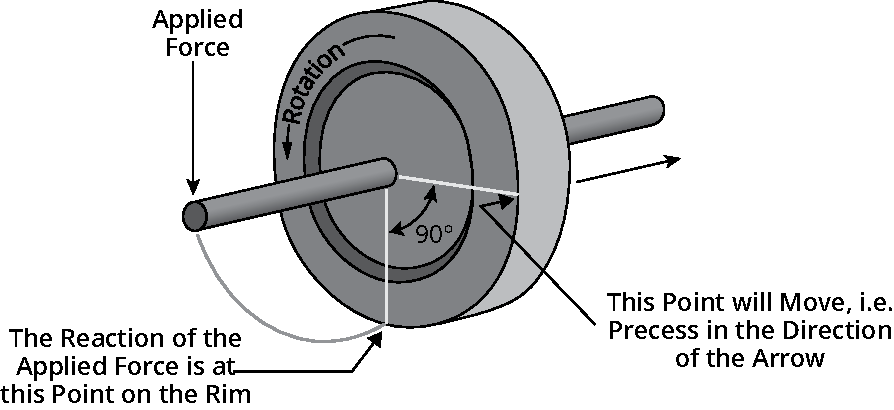
\includegraphics[width=0.4\columnwidth]{images/gyroscope_precession.pdf}
    \end{center}

    \only<1>{
    \begin{block}{Rigidez en el espacio}
        \begin{itemize}
            \item Al rotar, un giróscopo permanece en una posición fija en su plano de rotación, independientemente del movimiento de los soportes o el marco.
            \item La cantidad de \textbf{rigidez} que presenta el giróscopo es directamente proporcional a su velocidad de rotación (RPM) y su momento de inercia.
            \item Mayor velocidad de rotación, entonces mayor rigidez en el espacio.
            \item Mayor masa y radio efectivo, entonces mayor rigidez en el espacio.
        \end{itemize}
    \end{block}
    }
    \only<2>{
    \begin{block}{Movimiento dePrecesión}
        \begin{itemize}
            \item Toda fuerza aplicada perpendicularmente sobre el plano de rotación de un giróscopo se verá reflejada a $\SI{90}{\degree}$ en el sentido de la rotación.
            \item La magnitud de la precesión que pesenta el giróscopo es directamente proporcional a la fuerza aplicada e inversamente proporcional a la velocidad de rotación (RPM).
        \end{itemize}
    \end{block}
    }

    \note{Un trompo es un giróscopo! cuando esta por caerse muestra el efecto de precesión. La fuerza que se le aplica es la de la gravedad y hace que se mueva realizando una circunsferencia con su eje.}
\end{frame}


\begin{frame}
    \frametitle{Giróscopo MEMS (Microelectromechanical Systems)}
    \note{https://www.analog.com/en/technical-articles/mems-gyroscope-provides-precision-inertial-sensing.html}
    \footnotesize
    \begin{block}{Principio de Funcionamiento}
        Los giróscopos MEMS utilizan la fuerza de Coriolis, la fuerza tangencial experimentada por un objeto giratorio en movimiento radial.
    \end{block}

    \begin{figure}
        \subfloat[]
        {
            \movie[autostart,loop,poster]{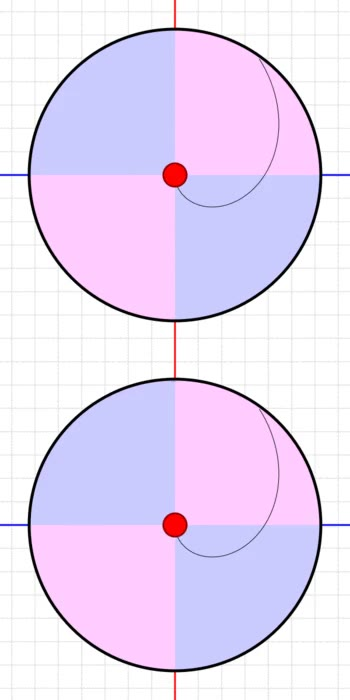
\includegraphics[width=0.19\columnwidth,valign=m]{./images/coriolis_force_video.jpg}}{./videos/coriolis_force.mp4}
        }
        \hspace{2em}
        \subfloat[]
        {
            \movie[autostart,loop,poster]{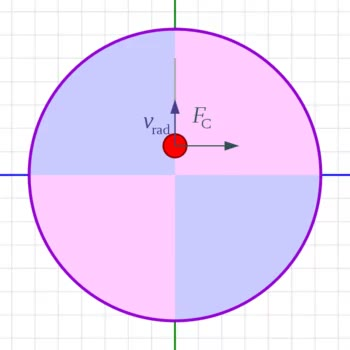
\includegraphics[width=0.2\columnwidth,valign=m]{./images/coriolis_force2_video.jpg}}{./videos/coriolis_force2.mp4}
        }
        \hspace{2em}
        \subfloat[]
        {
            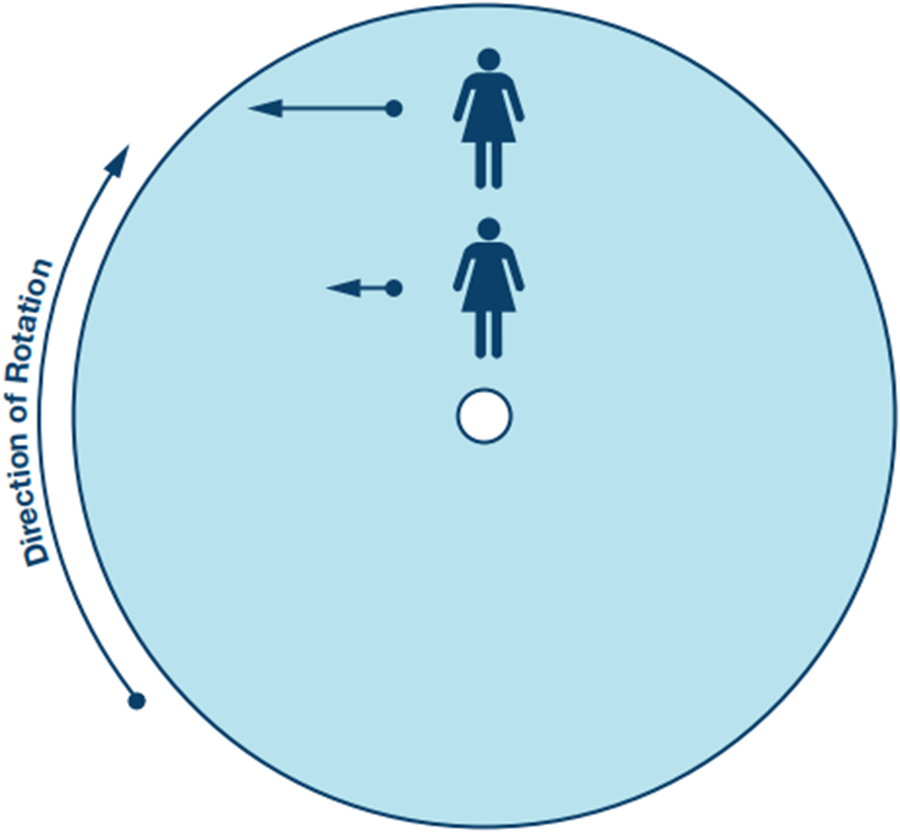
\includegraphics[width=0.2\columnwidth,valign=m]{images/gyroscope_mems_1.png}
        }
    \end{figure}

    Ejemplo de aceleración de Coriolis:
    Una persona que se mueve hacia el borde exterior Norte de una plataforma giratoria en sentido horario, debe aumentar el componente de velocidad hacia el Oeste (flechas azules) para mantener su rumbo hacia el Norte. La aceleración requerida es la \textbf{aceleración de Coriolis}.

    \note{Considérese parado en una plataforma giratoria, cerca del centro. Su velocidad relativa al suelo se muestra como la longitud de la flecha azul. Si tuviera que moverse a un punto cerca del borde exterior de la plataforma, su velocidad aumentaría en relación con el suelo, como lo indica la flecha azul más larga. La tasa de aumento de su velocidad tangencial, causada por su velocidad radial, es la aceleración de Coriolis.}

    \note{MEMS (sistemas microelectromecánicos) giroscopios son pequeños sensores, de bajo costo para medir la velocidad angular.  El sensor MEMS dentro de un giroscopio es muy pequeño (entre 1 a 100 micrómetros, el tamaño de un cabello humano).}

\end{frame}

\begin{frame}
    \frametitle{Giróscopo MEMS (Microelectromechanical Systems)}

    \note{https://www.analog.com/en/technical-articles/mems-gyroscope-provides-precision-inertial-sensing.html}
    
    \begin{itemize}
        \item Cuando se hace girar el giróscopo, una pequeña masa de resonancia se desplaza con los cambios de velocidad angular. Este movimiento se convierte en señales eléctricas de muy bajas corrientes que se pueden amplificar para ser leídas por un microcontrolador.
    \end{itemize}
    
    \begin{figure}[!h]
        \centering
        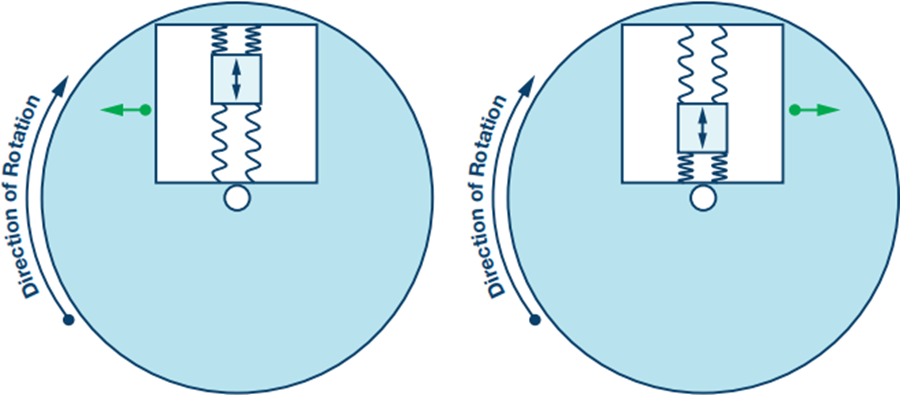
\includegraphics[width=0.4\columnwidth]{images/gyroscope_mems_2.png}
    \end{figure}
    
    \begin{itemize}
        \item Cuando la masa resonante se mueve hacia el borde exterior de la rotación, se acelera hacia la derecha y ejerce sobre el marco una fuerza de reacción hacia la izquierda (flecha verde). Cuando se mueve hacia el centro de la rotación, ejerce una fuerza hacia la derecha (flecha verde).
    \end{itemize}
    
\end{frame}

\begin{frame}
    \frametitle{Giróscopo MEMS (Microelectromechanical Systems)}
    \scriptsize
    \note{https://www.analog.com/en/technical-articles/mems-gyroscope-provides-precision-inertial-sensing.html}

    \begin{figure}[!h]
        \centering
        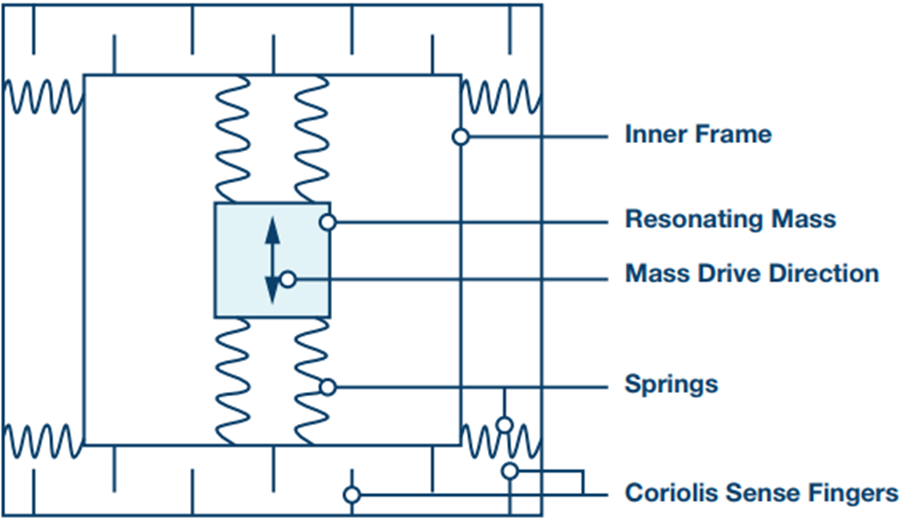
\includegraphics[width=0.5\columnwidth]{images/gyroscope_mems_structure.png}
        \caption{Estructura mecánica de un Giróscopo}
    \end{figure}

    \begin{itemize}
        \item Para medir la aceleración de Coriolis, el marco que contiene la masa resonante está sujeto a un marco externo por resortes a $\SI{90}{\degree}$ en relación con el movimiento resonante (de la masa). Esta figura también muestra los ``dedos'' de detección de Coriolis que se utilizan para detectar el desplazamiento de la trama mediante transducción capacitiva en respuesta a la fuerza ejercida por la masa.
    \end{itemize}
\end{frame}

\begin{frame}
    \frametitle{Giróscopo MEMS (Microelectromechanical Systems)}
    
    \note{https://www.analog.com/en/technical-articles/mems-gyroscope-provides-precision-inertial-sensing.html}
        
    \begin{itemize}
        \item A medida que la masa resonante se mueve y la superficie en la que está montado el giróscopo gira, la masa y su marco experimentan la aceleración de Coriolis, y se trasladan $\SI{90}{\degree}$ con respecto al movimiento vibratorio.
        
        \item A medida que aumenta la velocidad de rotación, también aumenta el desplazamiento de la masa y la señal derivada de la capacitancia correspondiente cambia.
    \end{itemize}
    
    \begin{center}
        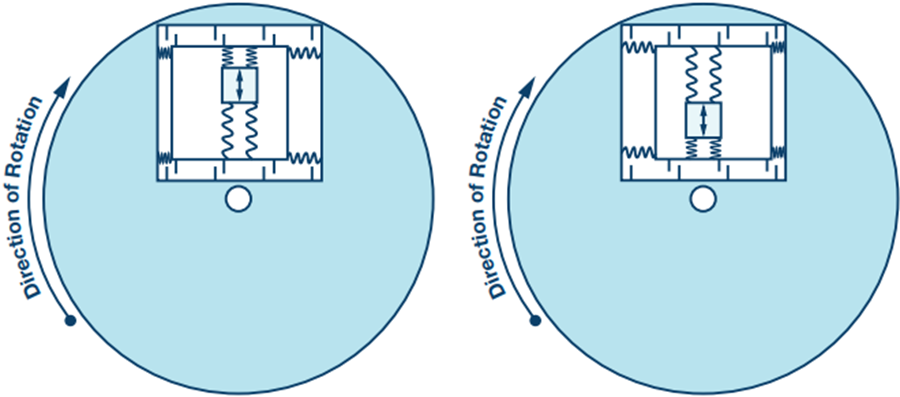
\includegraphics[width=0.5\columnwidth]{images/gyroscope_mems_3.png}
    \end{center}

\end{frame}

\begin{frame}
    \frametitle{Acelerómetro}
    
    \begin{figure}[!h]
    	\subfloat[]
        {
            \movie[autostart,loop,poster]{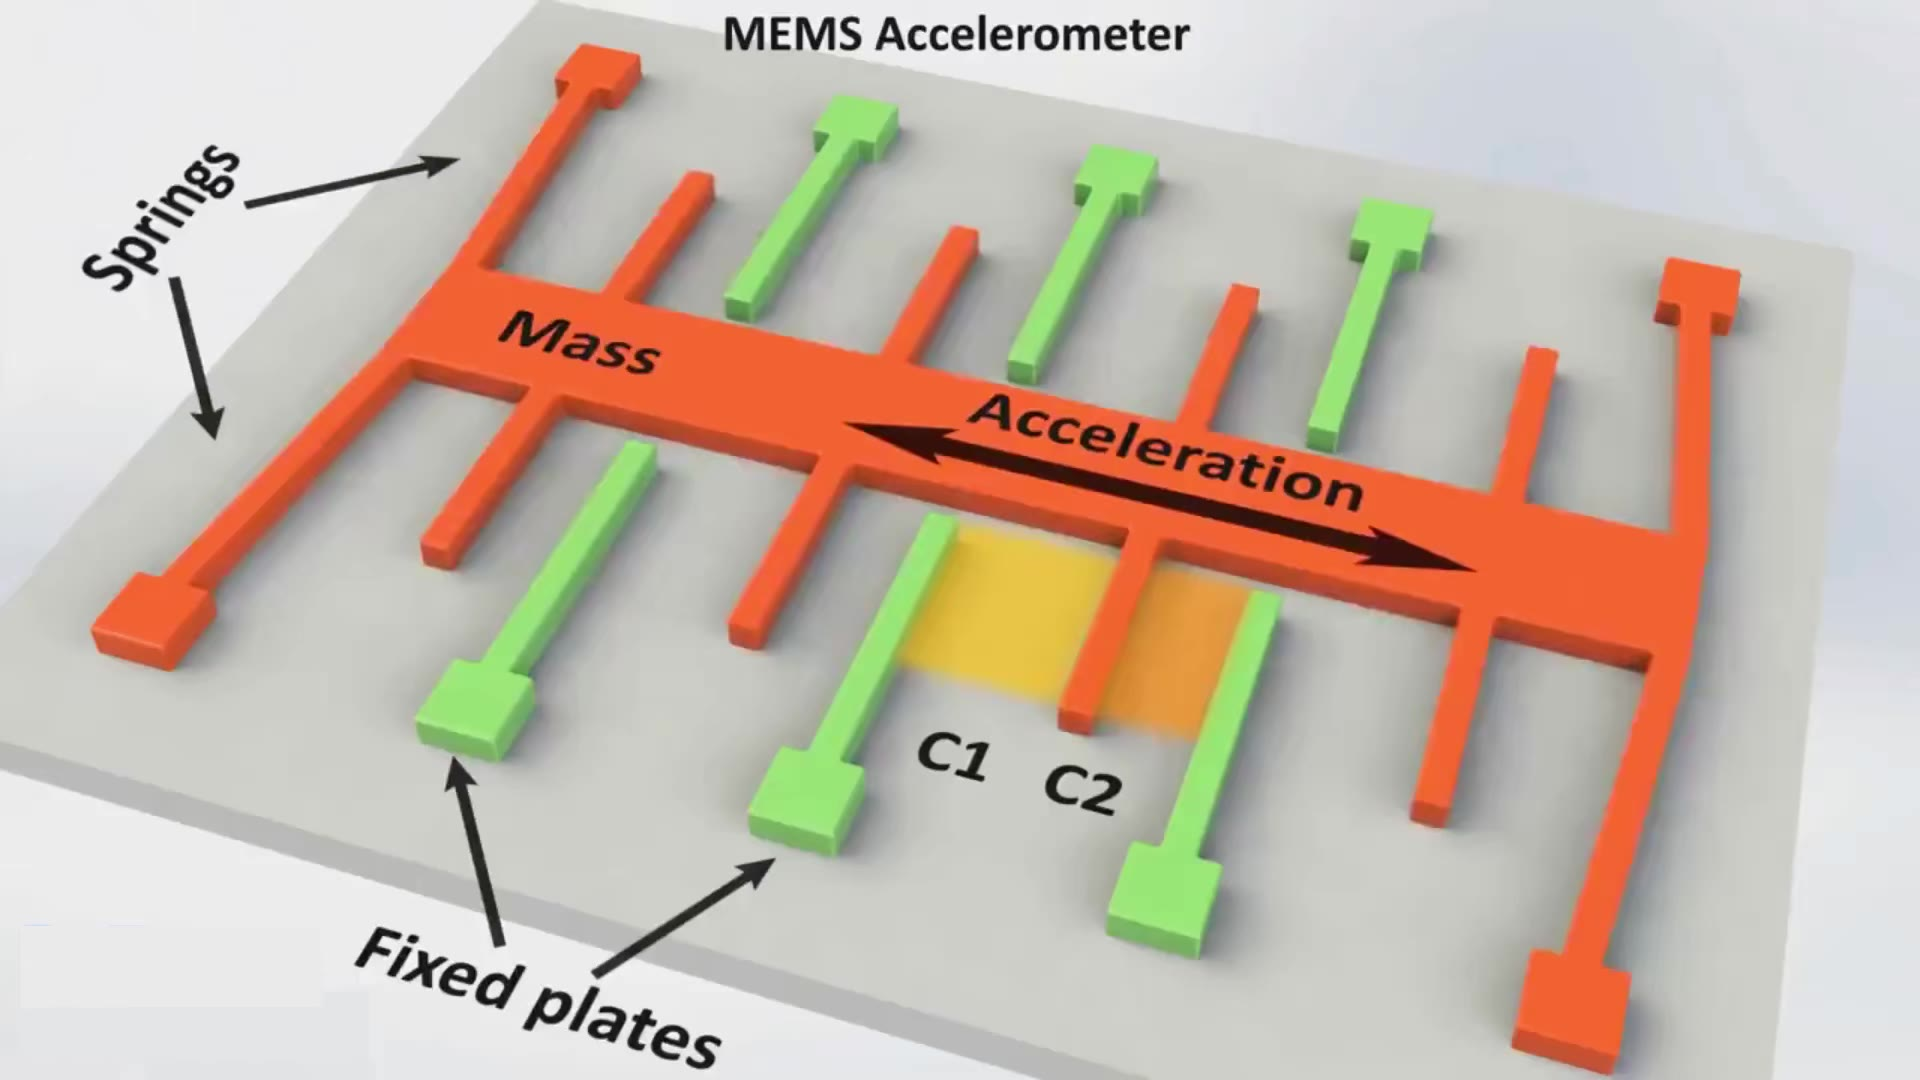
\includegraphics[width=0.3\columnwidth,valign=m]{./images/accelerometer_mems_video.jpg}}{./videos/accelerometer_mems.mp4}
        }
        \hspace{1em}
    	\subfloat[]
    	{
    		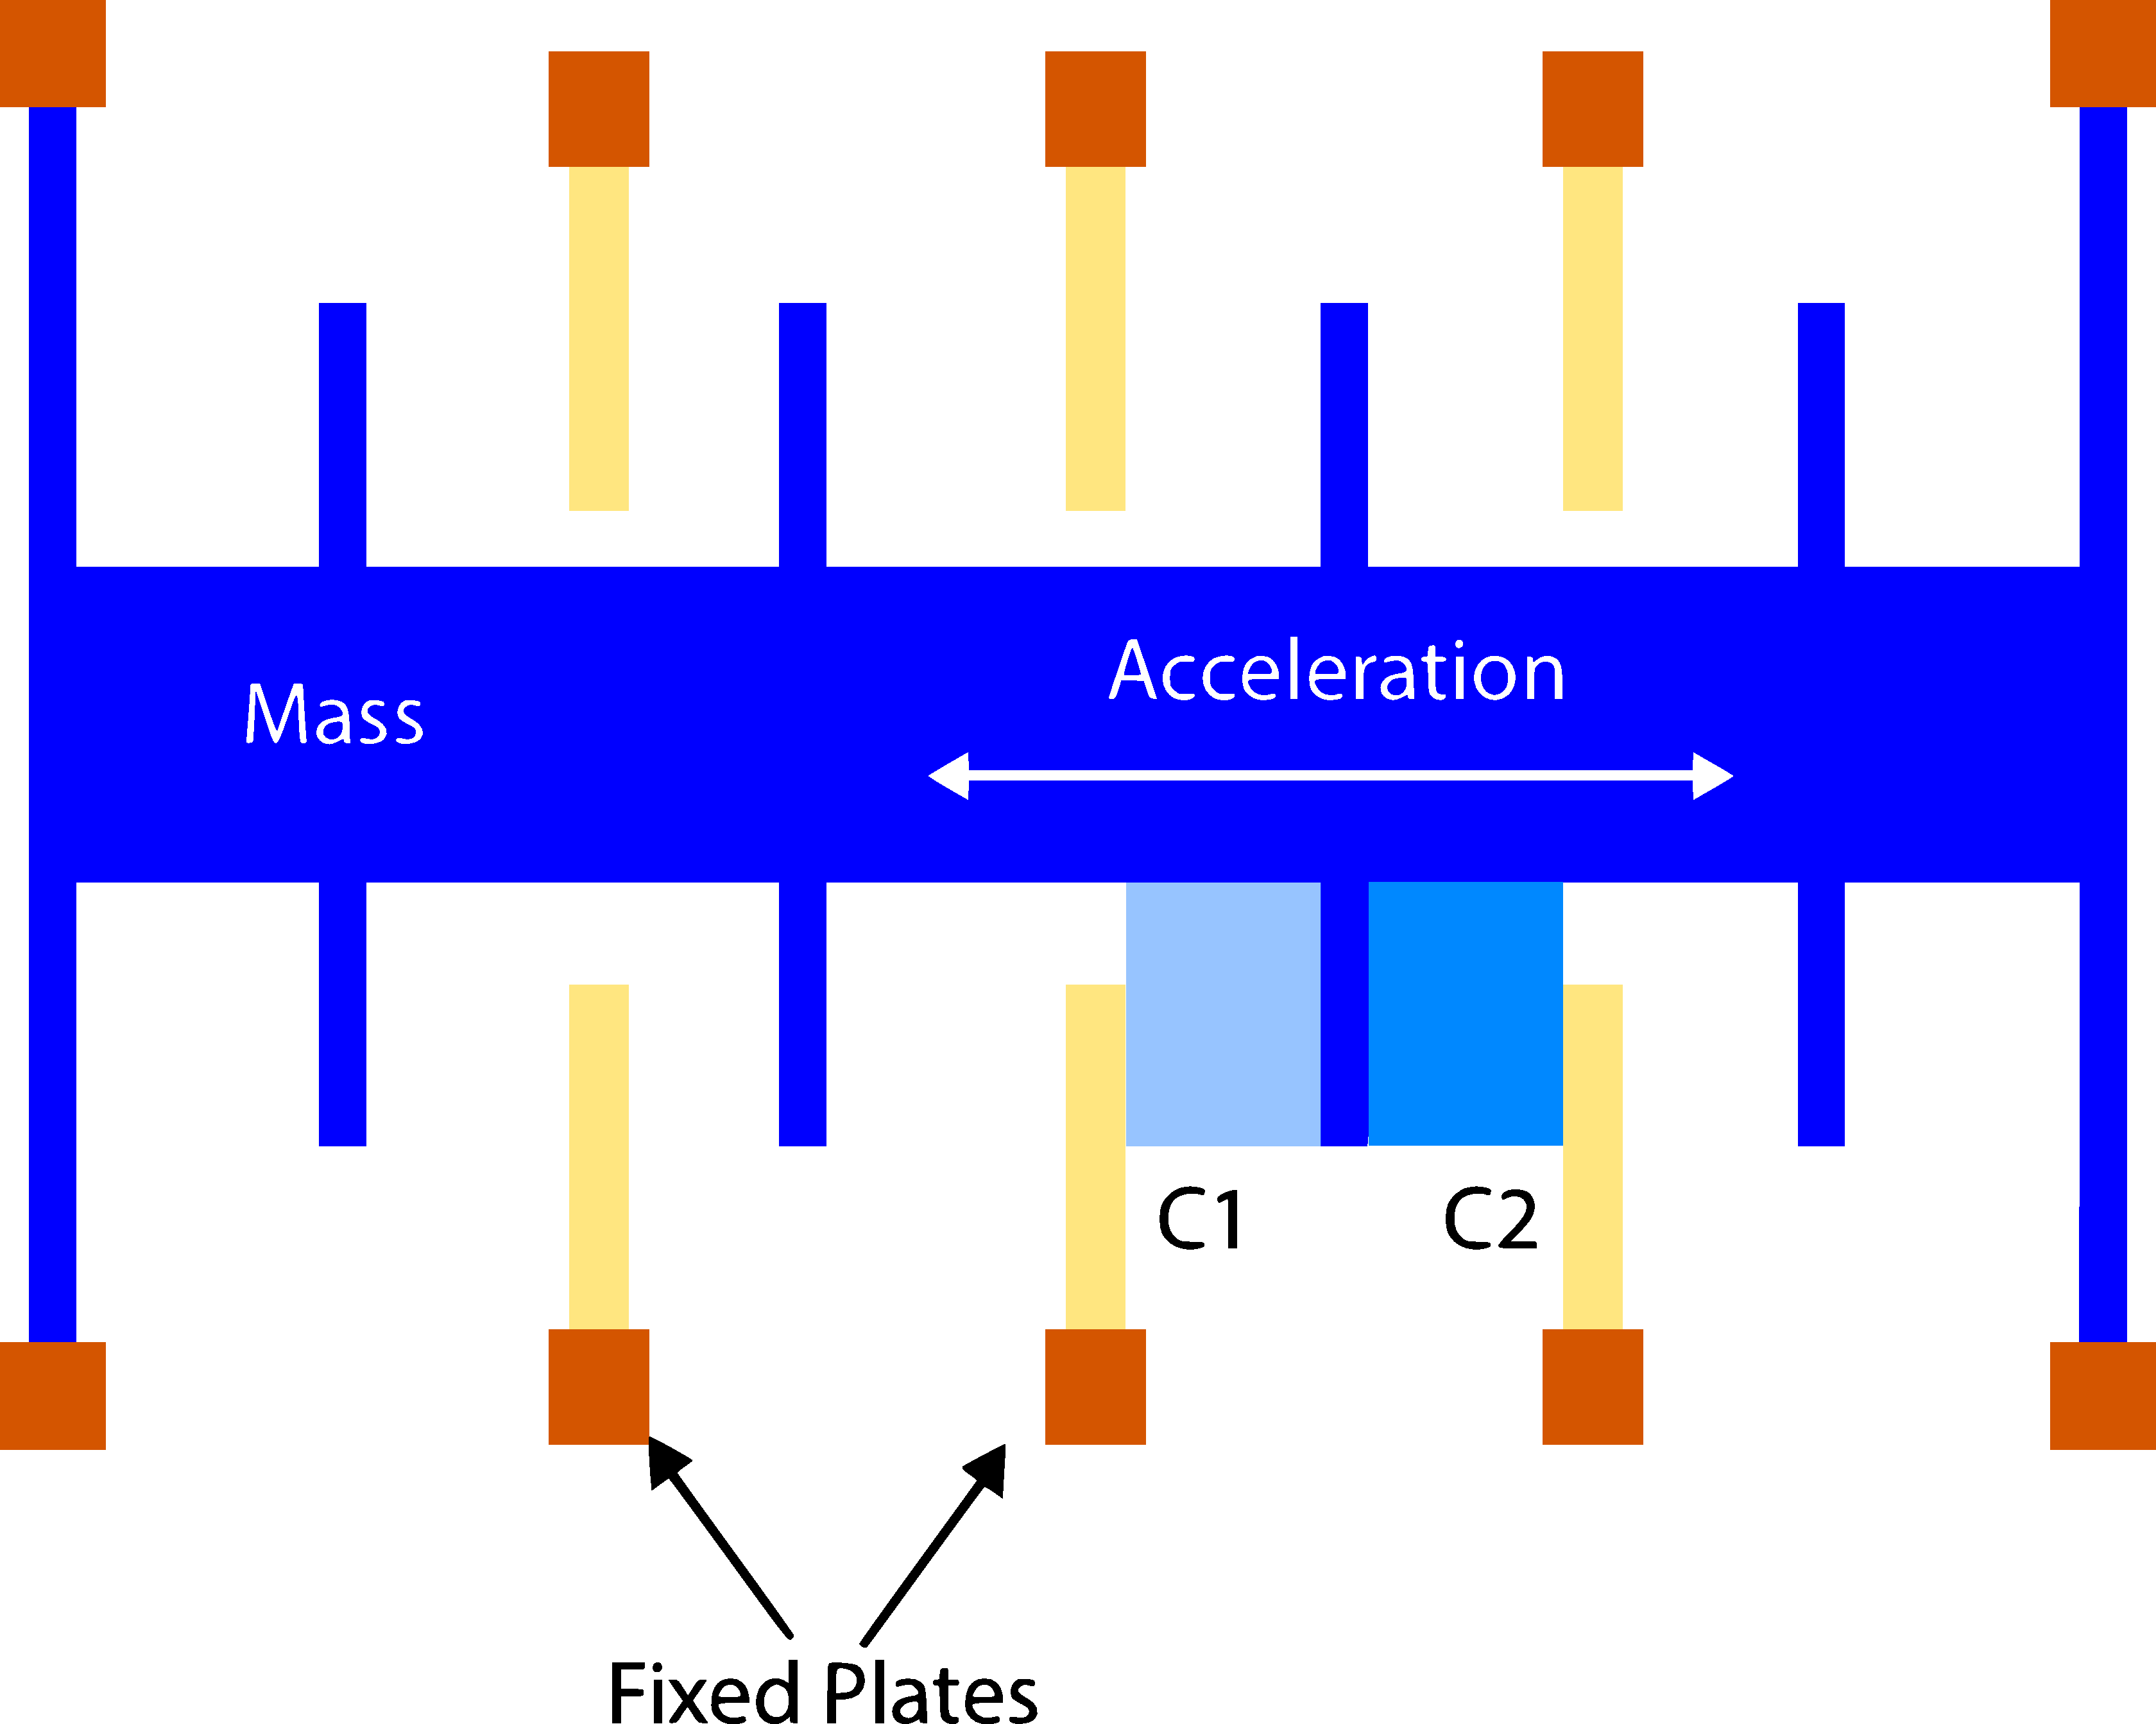
\includegraphics[width=0.2\columnwidth,valign=m]{images/accelerometer_mems.pdf}
    	}
        \hspace{1em}
    	\subfloat[]
    	{
    		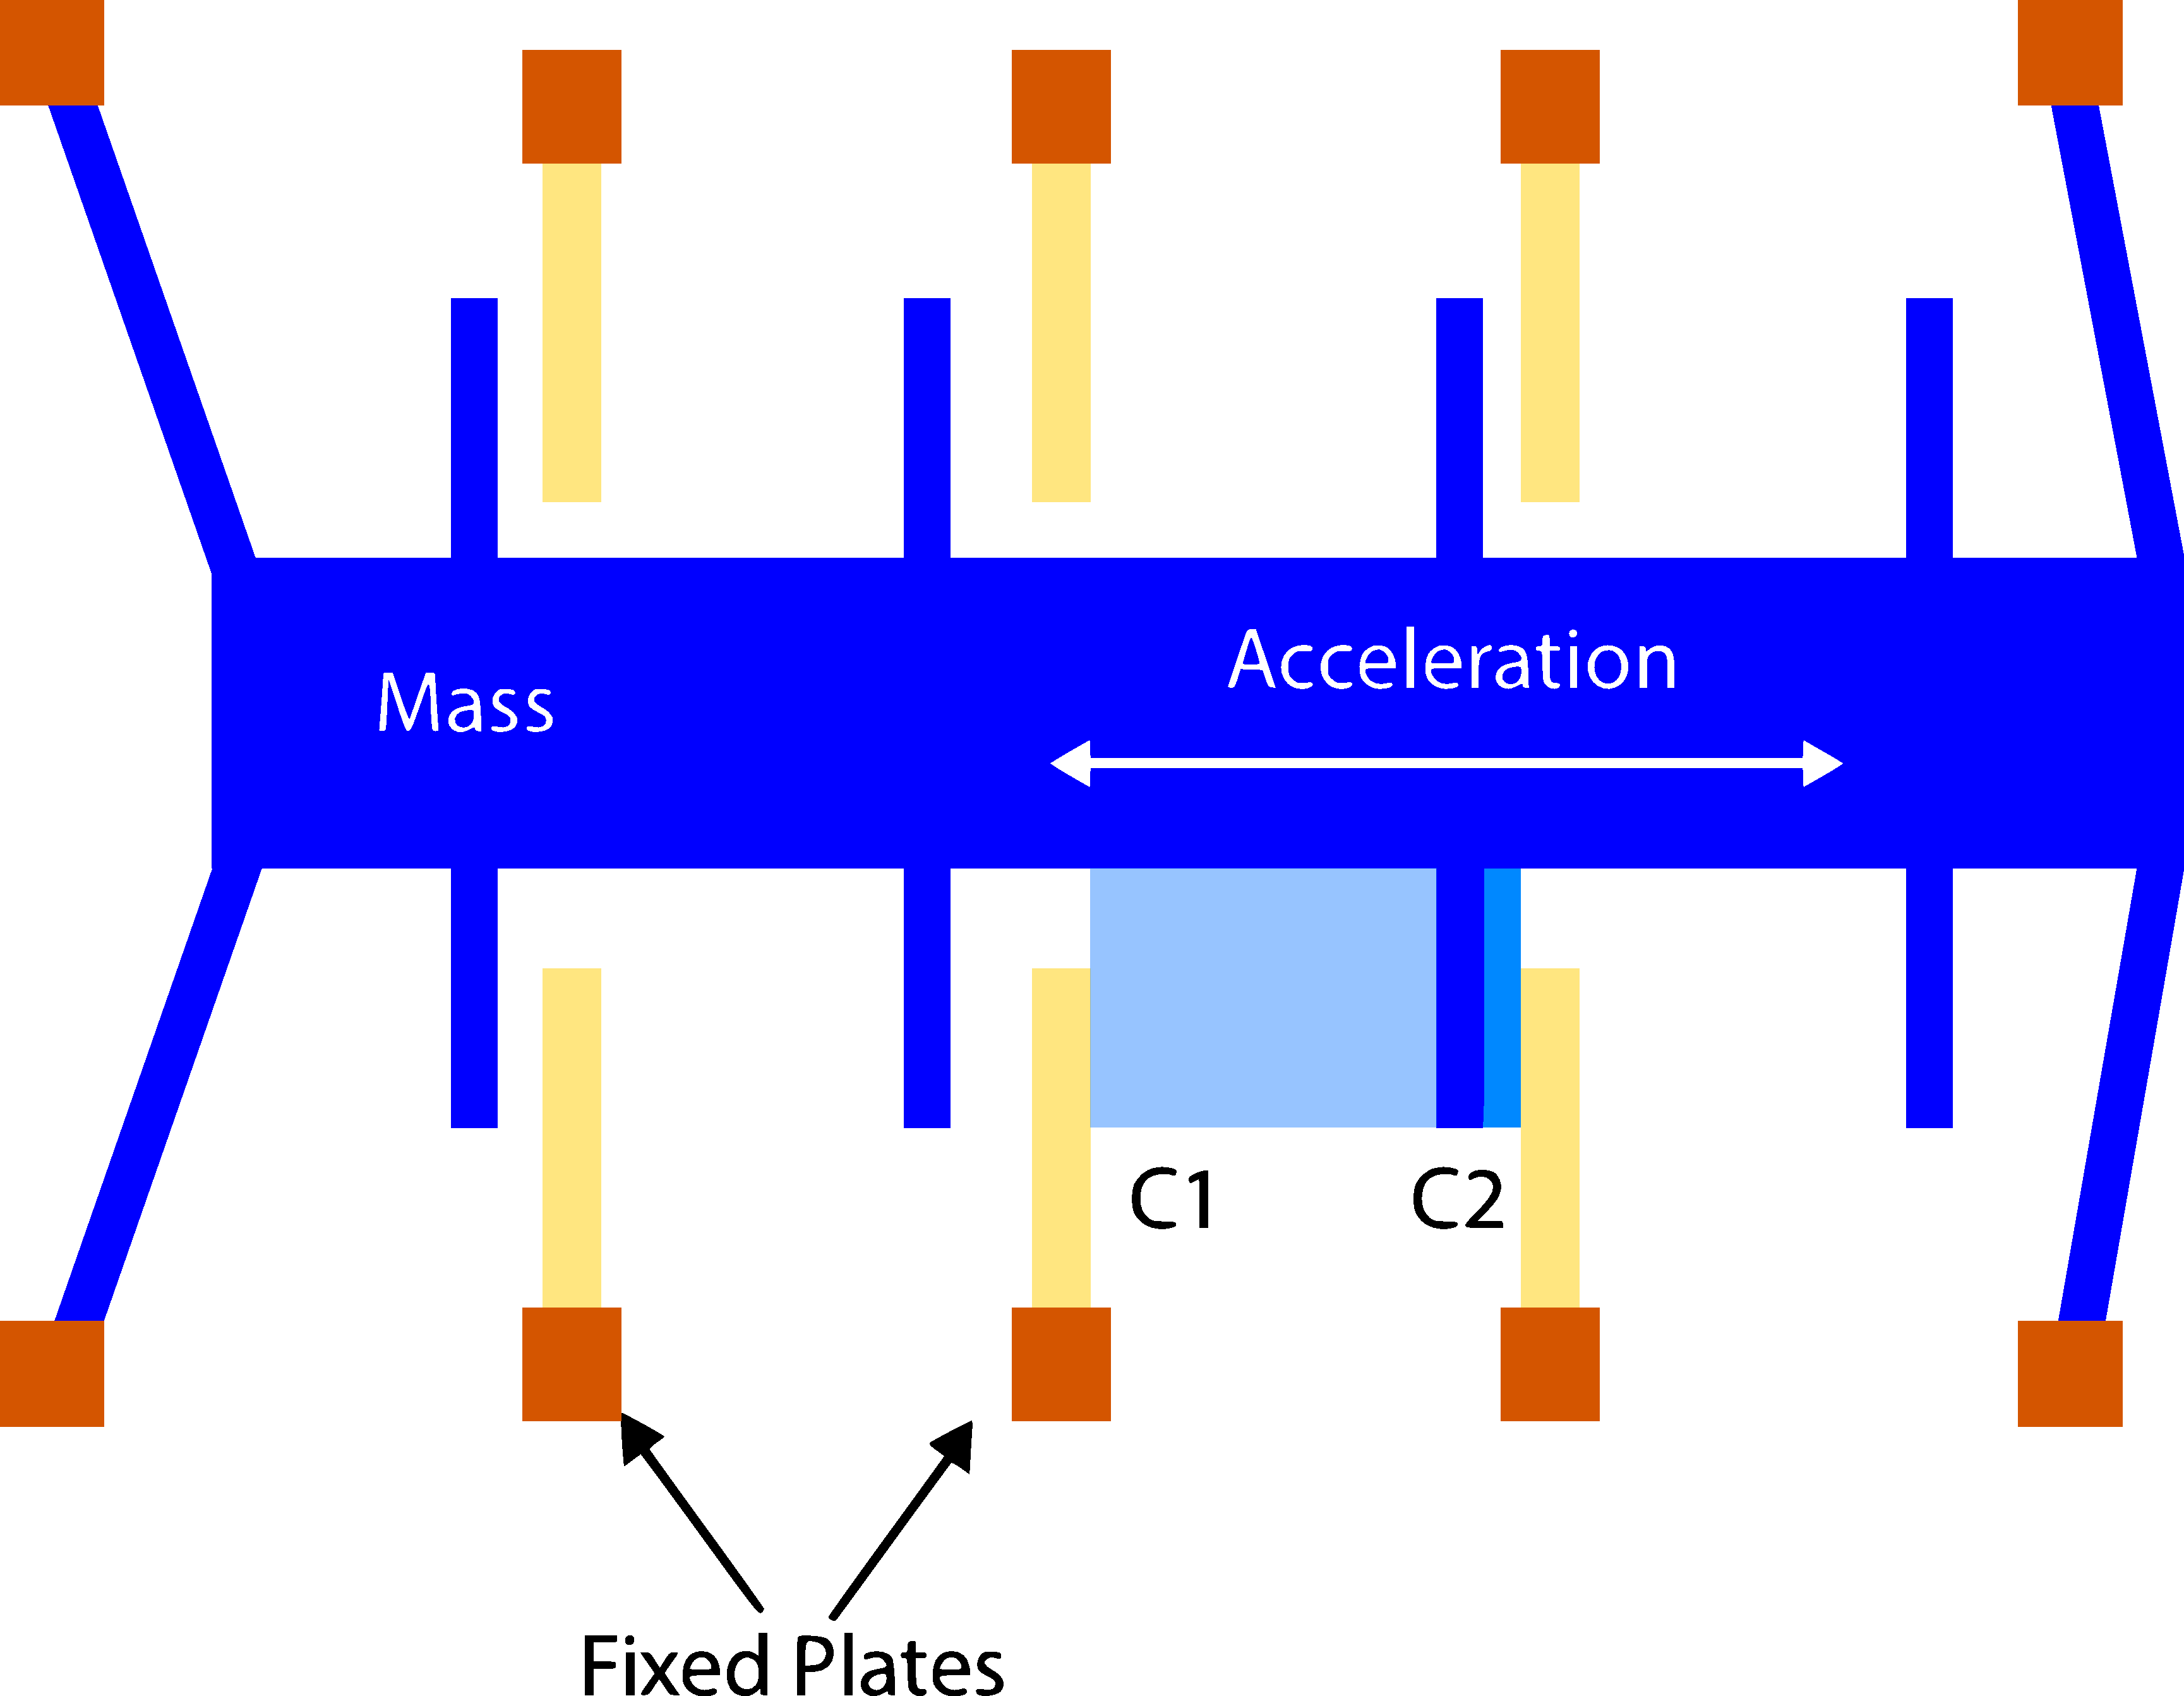
\includegraphics[width=0.2\columnwidth,valign=m]{images/accelerometer_mems2.pdf}
    	}
    \end{figure}
    \scriptsize
    \begin{block}{Principio de Funcionamiento}
        Mide la aceleración midiendo el cambio en la capacitancia. Tiene una masa unida a un resorte que se limita a moverse en una dirección y placas exteriores fijas. Entonces, cuando se aplica una aceleración, la masa se mueve y la capacitancia entre las placas y la masa cambiará. Este cambio de capacitancia es medido, y se corresponde a un valor de aceleración particular.
    \end{block}
    
    \begin{itemize}
        \item Introceptivo
        \item Pasivo
        \item Mide aceleración
        \item Unidad de medición $\si{\meter\per\square\second}$
    \end{itemize}
    
\end{frame}

\begin{frame}
    \frametitle{IMU (Inertial Measurement Unit)}
    \note{página 122 del libro Introduction to autonomous mobile robots 2nd edition}
    
    \begin{figure}[!h]
            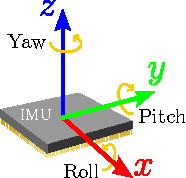
\includegraphics[width=0.2\columnwidth]{images/imu.pdf}
    \end{figure}
    
    \begin{itemize}
        \item 3 giróscopos ortogonales y 3 acelerómetros ortogonales.
        \item Permite estimar: posición, orientación, velocidad lineal, velocidad angular y aceleración 
        \item La orientación se obtiene integrando el giróscopo en el tiempo
        \item La velocidad lineal se obtiene integrando el acelerómetro en el tiempo
        \item La posición se obtiene integrando la velocidad en el tiempo
        \item \textbf{Debido a que los datos del acelerómetro se integran dos veces para obtener la posición, cualquier error residual da como resultado un error cuadrático en la posición}
        \item Mediciones absolutas (GPS o cámaras) permiten cancelar esta deriva de error.
    \end{itemize}
    
    \note{
    Una unidad de medida inercial (IMU) es un dispositivo que utiliza giroscopios y acelerómetros para estimar la posición relativa, la velocidad y la aceleración de un vehículo en movimiento. Una IMU también se conoce como Sistema de Navegación Inercial (INS).
    Una IMU estima la pose de seis grados de libertad (DOF) del vehículo: posición (x, y, z) y orientación (pitch, yaw, roll). También estima velocidad y aceleración.
    
    Los datos del giroscopio se integran para estimar la orientación del vehículo, mientras que los tres acelerómetros se utilizan para estimar la aceleración instantánea del vehículo. A continuación, la aceleración se transforma en el marco de navegación local por medio de la estimación actual de la orientación del vehículo en relación con la gravedad. En este punto, el vector de gravedad se puede restar de la medición. Luego, la aceleración resultante se integra para obtener la velocidad y luego se integra nuevamente para obtener la posición, siempre que tanto la velocidad inicial como la posición sean conocidas a priori. Para superar la necesidad de conocer la velocidad inicial, la integración generalmente comienza en reposo (es decir, velocidad igual a cero).
    
    Observe que las IMU son extremadamente sensibles a los errores de medición tanto en giroscopios como en acelerómetros. Por ejemplo, la deriva en el giroscopio socava inevitablemente la estimación de la orientación del vehículo en relación con la gravedad, lo que da como resultado una cancelación incorrecta del vector de gravedad. Además, observe que, debido a que los datos del acelerómetro se integran dos veces para obtener la posición, cualquier vector de gravedad residual da como resultado un error cuadrático en la posición. Debido a esto y al hecho de que cualquier otro error se integra con el tiempo, la deriva es un problema fundamental en las IMU. Después de un largo período de funcionamiento, todas las IMU se desvían. Para cancelar esta deriva, se requiere alguna referencia a alguna medida externa.
    }
\end{frame}



\begin{frame}
    \frametitle{Modelo de cámara Pinhole}
    
    \begin{figure}[!h]
        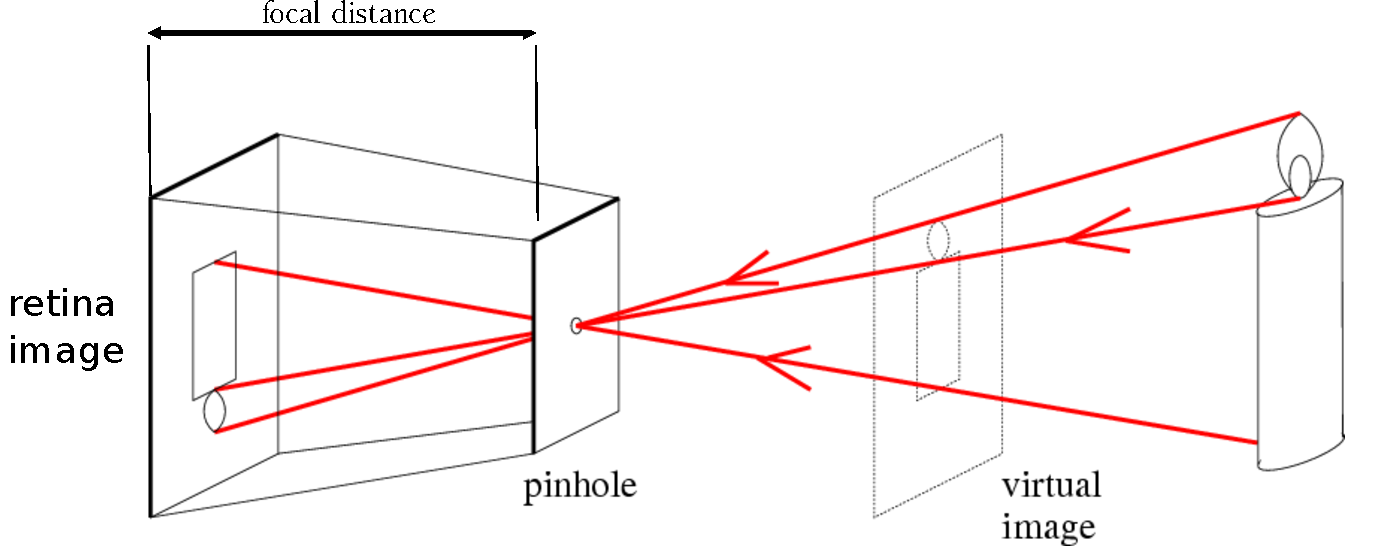
\includegraphics[width=0.6\columnwidth]{images/pinhole_camera_virtual_image.pdf}
    \end{figure}   
\end{frame}

\begin{frame}
    \frametitle{Modelo de cámara Pinhole}
    \scriptsize
    \begin{figure}[!h]
        \subfloat[]
        {
            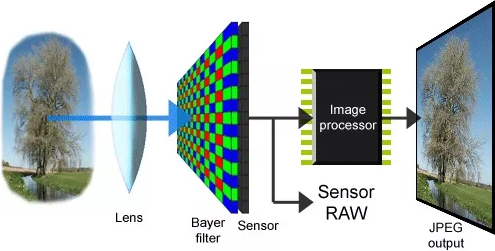
\includegraphics[width=0.55\columnwidth]{images/camera_sensor.png}
        }
        \subfloat[]
        {
            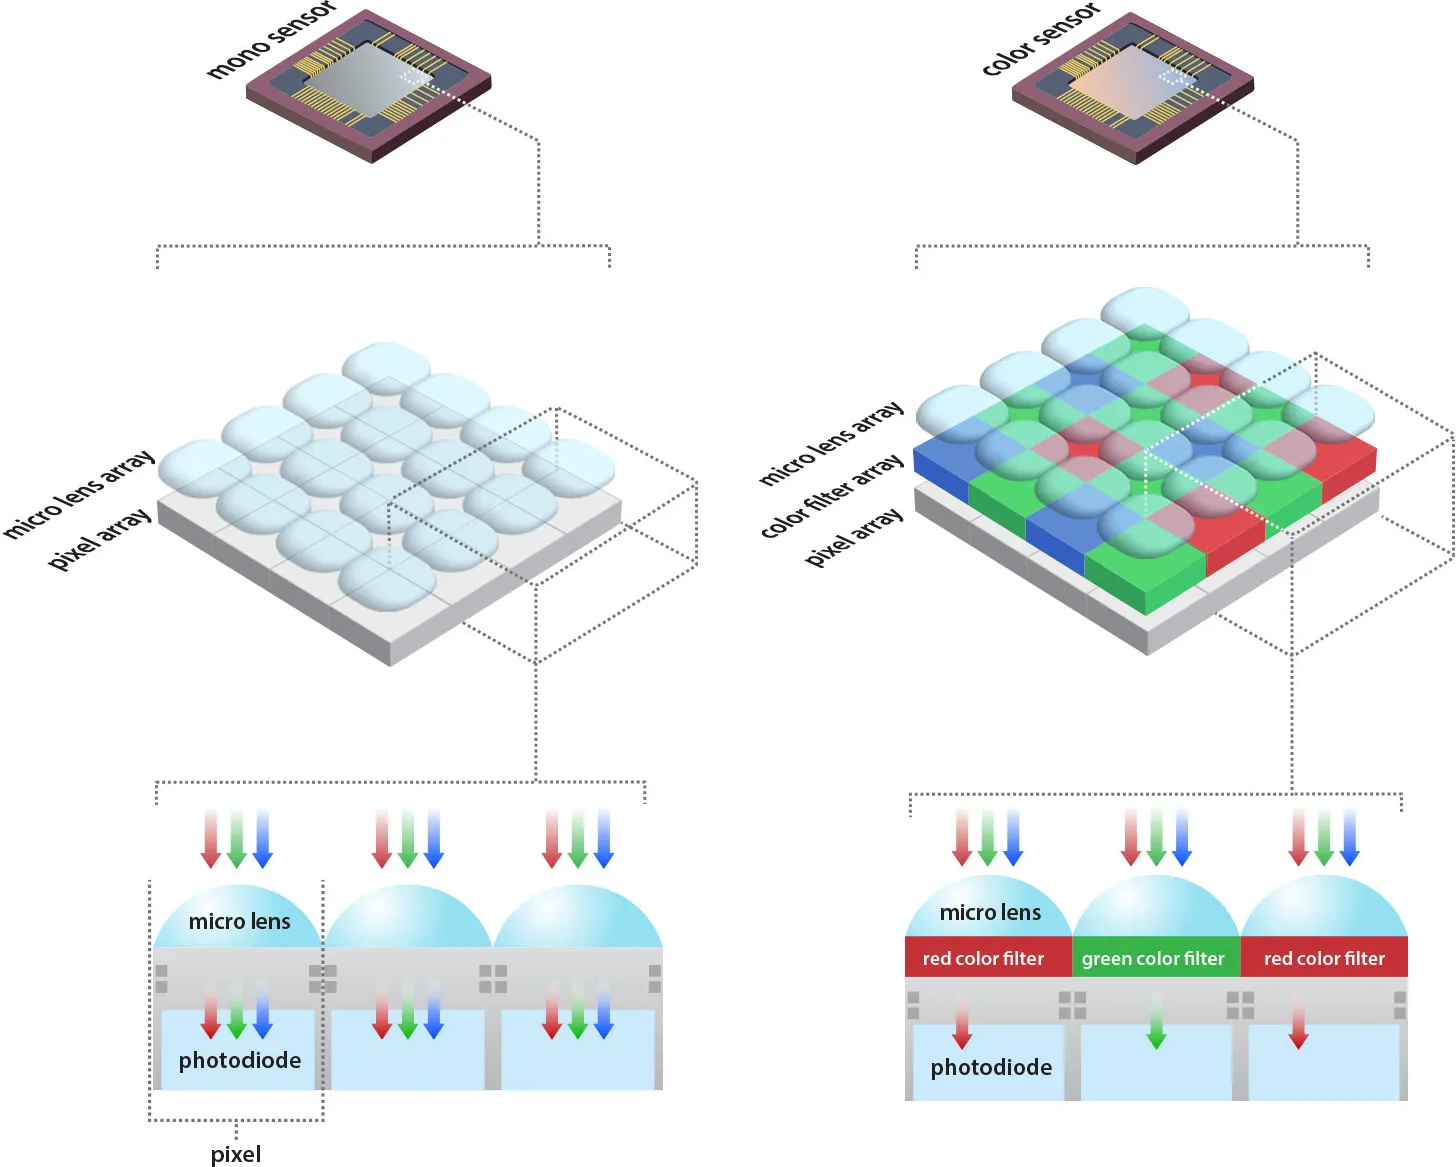
\includegraphics[width=0.4\columnwidth]{images/camera_color_mono_bayer_pattern.png}
        }
    \end{figure}

    \begin{itemize}
        \item Exteroceptivo
        \item Pasivo
        \item Capturan gran cantidad de información (información semántica)
        \item Las imágenes presentan blur ante movimientos rápidos o de poca luz
        \item Requiere escenas bien iluminadas
    \end{itemize}

\end{frame}


\begin{frame}
    \frametitle{Imagen}
    
    \begin{figure}[!h]
        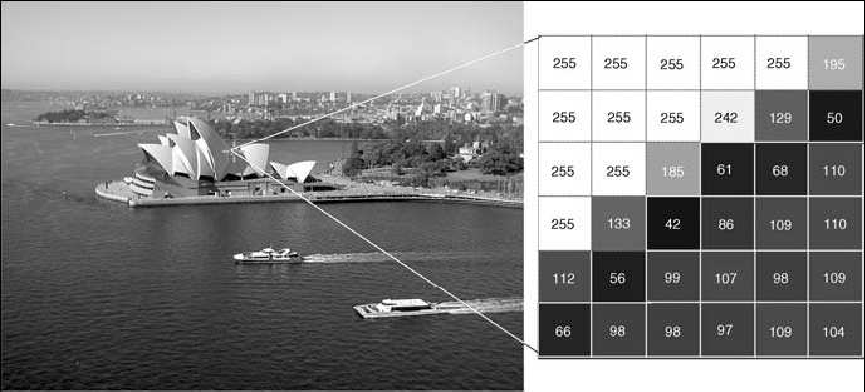
\includegraphics[width=0.4\columnwidth]{images/camera_grayscale_image_pixels.pdf}
    \end{figure}   
    
    \begin{columns}
    	\begin{column}{0.5\textwidth}
		    \begin{figure}[!h]
			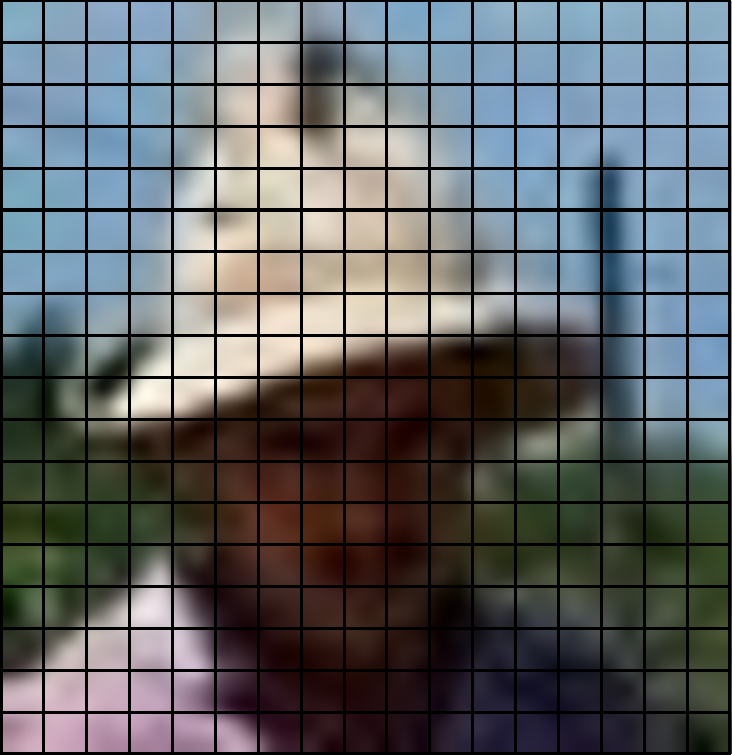
\includegraphics[width=0.4\columnwidth]{images/image_pixels.pdf}
			\end{figure}
    	\end{column}
    	\begin{column}{0.3\textwidth}
		Imagen color tiene 3 canales: R, G y B.
		\begin{equation*}
			f(x,y)=
			\begin{bmatrix}
				r(x,y) \\
				g(x,y) \\
				b(x,y)
			\end{bmatrix}
		\end{equation*}
    	\end{column}
    \end{columns}
\end{frame}



\begin{frame}
    \frametitle{Cámara Time of Flight}
    \note{https://en.wikipedia.org/wiki/Time-of-flight_camera}
    
    \begin{block}{Principio de funcionamiento}
        Funciona de manera similar a un lidar con la ventaja de que toda la escena 3D se captura al mismo tiempo y que no hay partes móviles. Este dispositivo utiliza una fuente de luz infrarroja modulada para determinar la distancia de cada píxel de un sensor Photonic Mixer Device (PMD).
    \end{block}
    
    \begin{itemize}
        \item Esteroceptivo
        \item Activo
       
    \end{itemize}
    
\end{frame}

\begin{frame}
    \frametitle{Láser 2D}

    \note{https://cdn.sick.com/media/docs/3/43/443/operating_instructions_lms1104c_111031s01_2d_lidar_sensors_en_im0079443.pdf}
    
    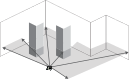
\includegraphics[width=0.4\columnwidth]{images/lidar_example.}

\end{frame}

\begin{frame}
    \frametitle{Láser 3D}

\end{frame}

\begin{frame}
    \frametitle{Sensor Ultrasónico}
    \scriptsize
    
    \begin{center}
        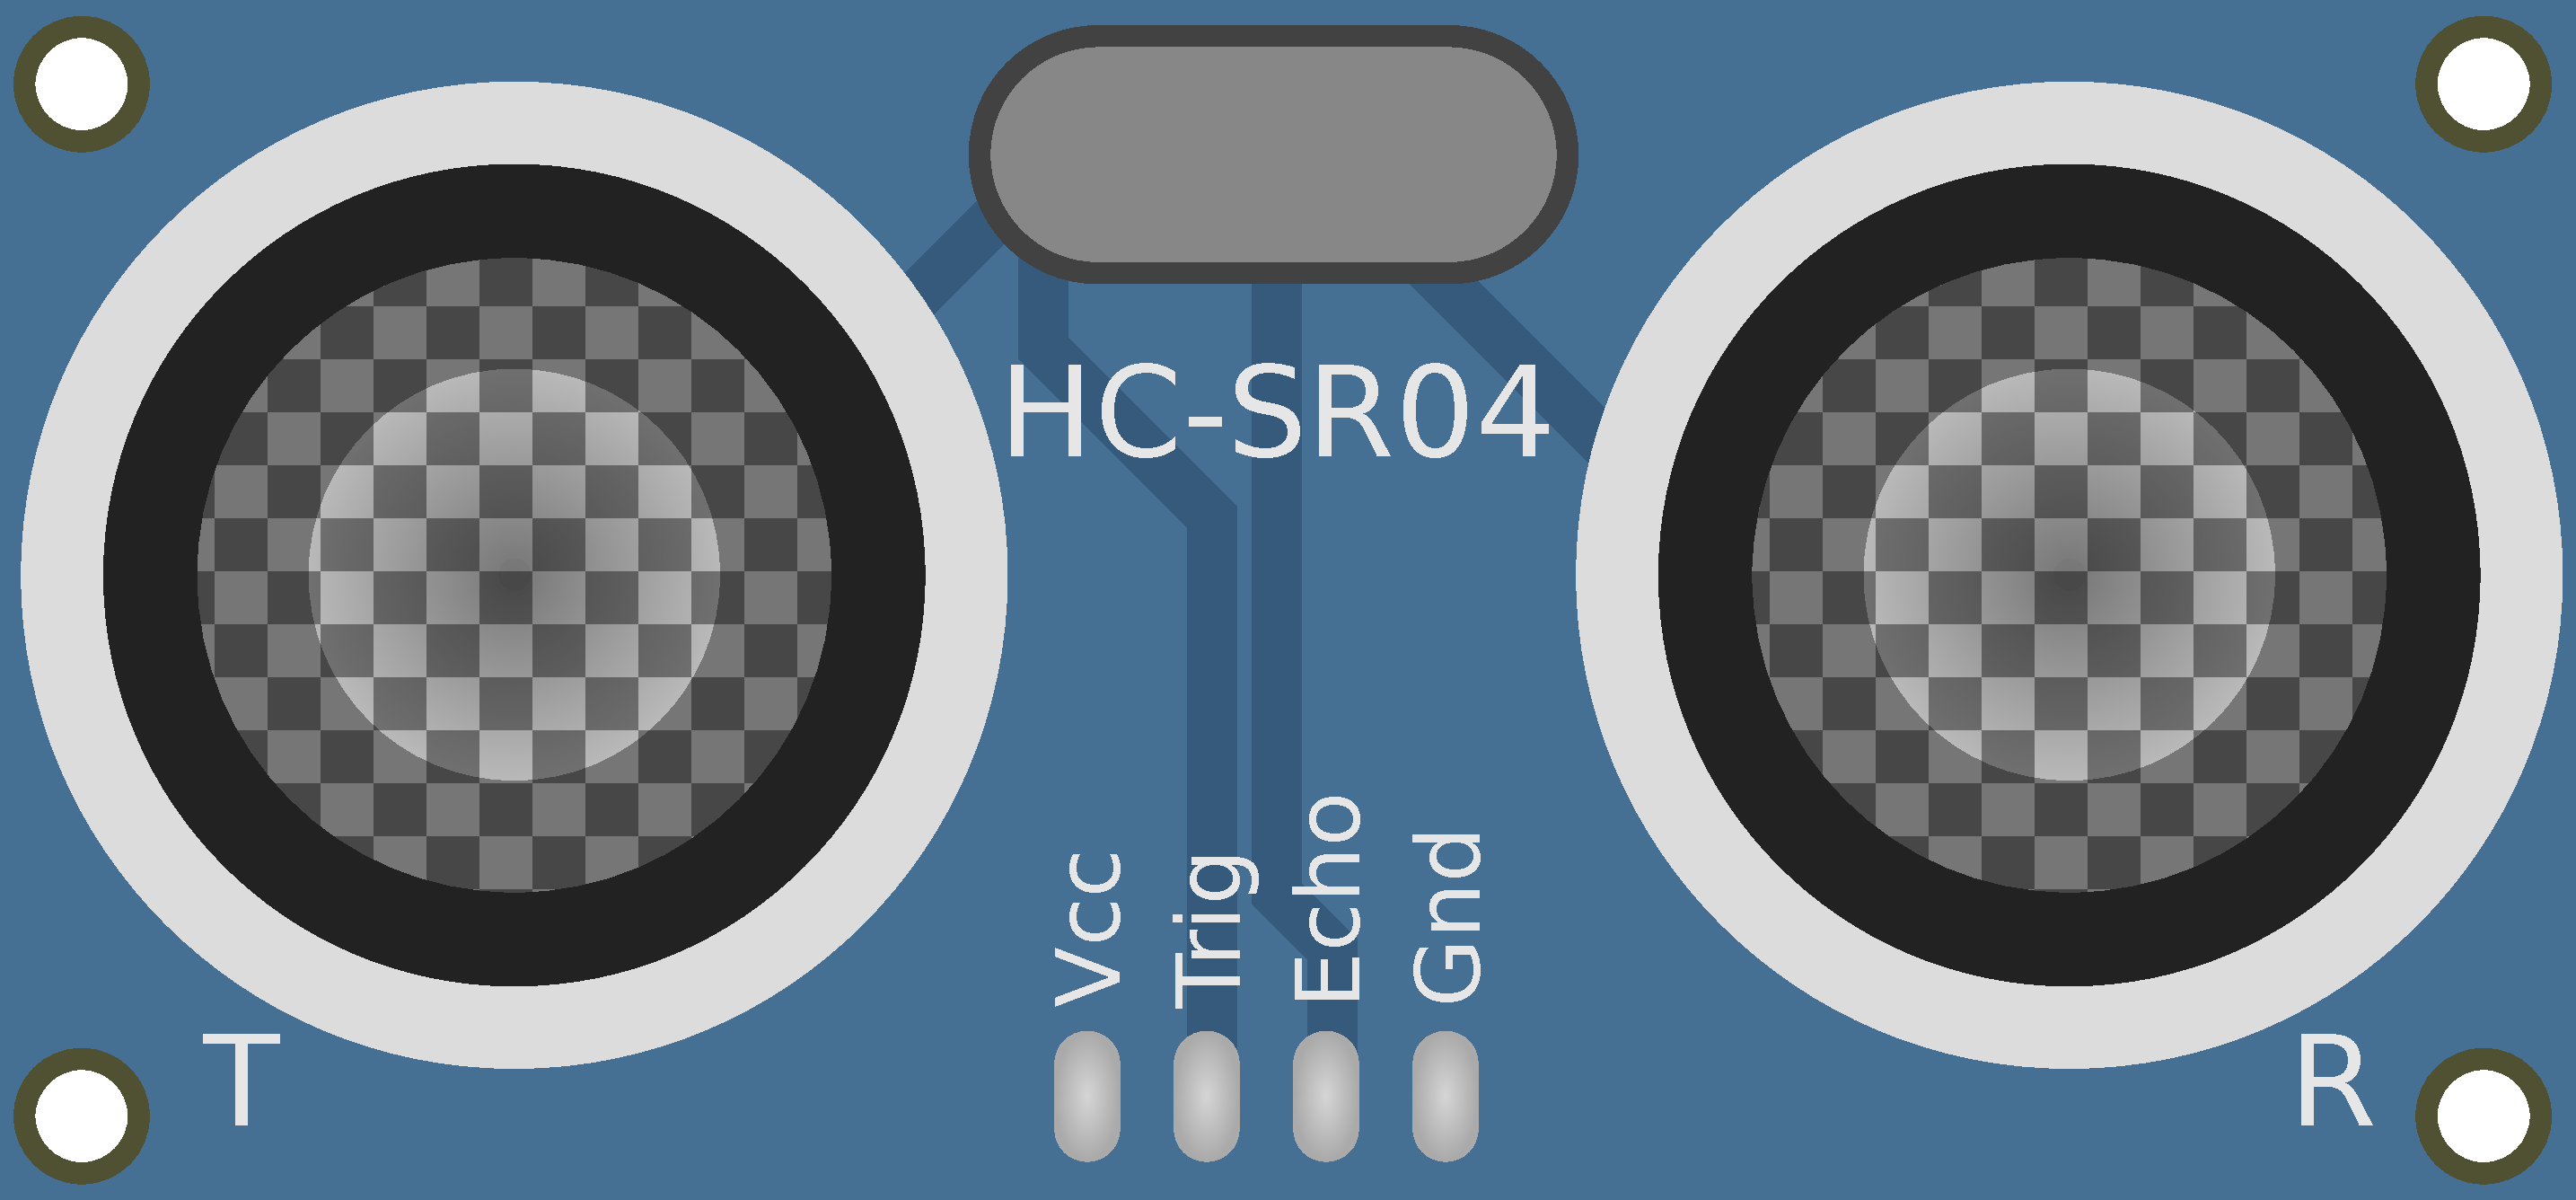
\includegraphics[width=0.2\columnwidth]{images/ultrasonic_sensor.pdf}
    \end{center}
    
    
    \begin{block}{Principio de funcionamiento}
        El principio básico de un sensor ultrasónico es transmitir un paquete de ondas de presión (ultrasónicas) y medir el tiempo que tarda este paquete de ondas en reflejarse y regresar al receptor. La distancia del objeto que causa el reflejo  $d$ se puede calcular en función de la velocidad de propagación del sonido $c$ y el tiempo de vuelo $t$.
   
        \begin{equation*}
            d = \dfrac{c t}{2}
        \end{equation*}
        La velocidad del sonido está dada por
        \begin{equation*}
            c = \sqrt{\gamma R T}
        \end{equation*}
        donde
        \begin{itemize}
            \item $\gamma$ es el ratio de calores específicos\\
            \item $R$ es la constante del gas\\
            \item $T$ es la temperatura del ambiente en grados Kelvin
        \end{itemize}
            
        En aire a presión estándar y $\SI{20}{\degree}$ la velocidad del sonido es aproximadamente $c = \SI{343}{\meter\over\second}$.
    \end{block}
\end{frame}

\begin{frame}
    \frametitle{Sensor de triangulación óptica}

    \begin{figure}[!h]
    \centering
    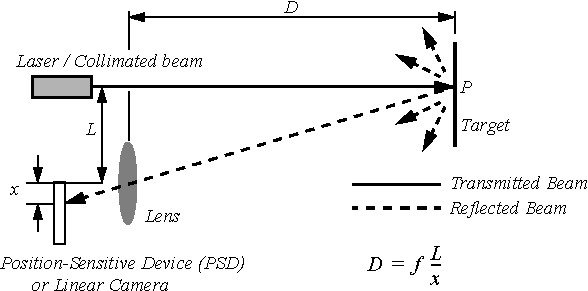
\includegraphics[width=0.7\columnwidth]{images/optical_triangulation.pdf}
    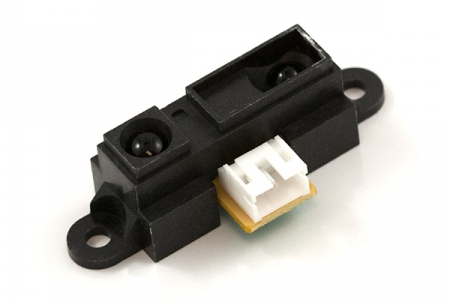
\includegraphics[width=0.25\columnwidth]{images/optical_triangulation.png}
    \end{figure}
    
\end{frame}

\begin{frame}
    \frametitle{Cámara de luz estructurada}
    \small
    \begin{center}
        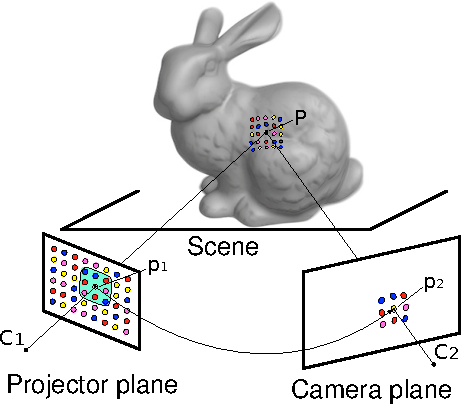
\includegraphics[width=0.4\columnwidth]{images/structured_light.pdf}
    \end{center}

    \begin{block}{Principio de funcionamiento}
        La luz estructurada (\emph{structured light}) es el proceso de proyectar un patrón conocido de píxeles (ocasionalmente rejillas o barras horizontales) en una escena. La manera en que dicho patrón se deforma cuando golpea distintas superficies permite a los sistemas de visión calcular la profundidad e información de la superficie de los objetos en la escena.
    \end{block}


\end{frame}

\begin{frame}
    \frametitle{GNSS (Global Navigation Satellite System) - Single Point Positioning (SPP)}
     \note{Página que explica como funciona un GNSS http://gutovnik.com/como_func_sist_gps.html}
     \note{video explicativo: https://youtu.be/U3eX6QKS9kY}
     \note{Slides de la estación permanente de la UNR: https://www.fceia.unr.edu.ar/gps/extension/GPSenTiempoReal.pdf}

     \begin{figure}[!h]
        \centering
        \subfloat[]
        {
            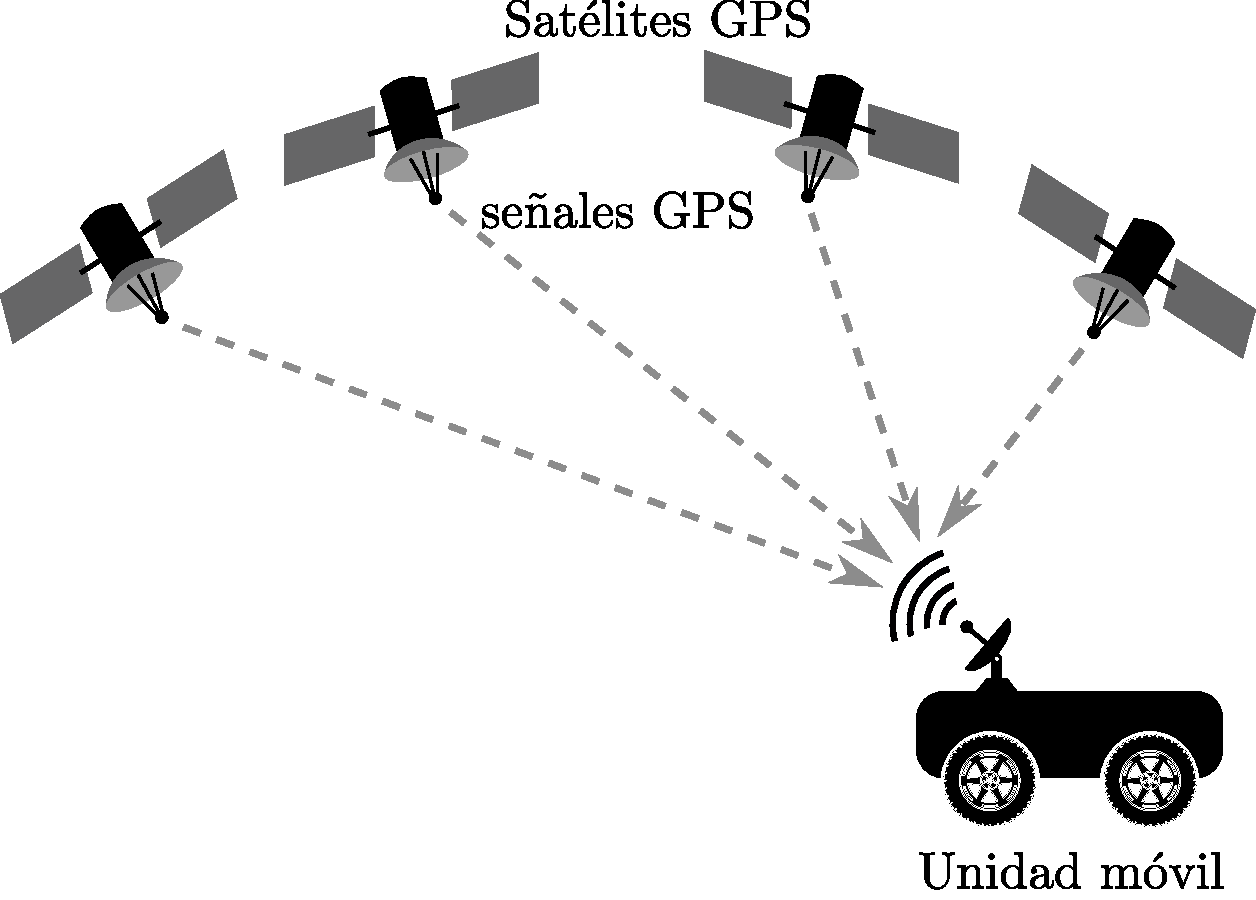
\includegraphics[width=0.2\columnwidth,valign=m]{gnss.pdf}
        }
        \hspace*{1cm}
        \subfloat[]
        {
            \movie[autostart,loop,poster]{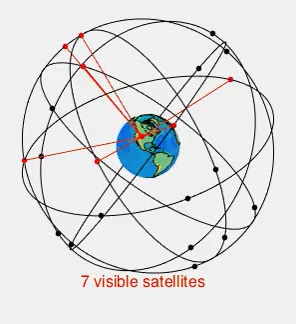
\includegraphics[width=0.17\columnwidth,valign=m]{./images/gnss_video.jpg}}{./videos/gnss.mp4}
        }
        \subfloat[]
        {
            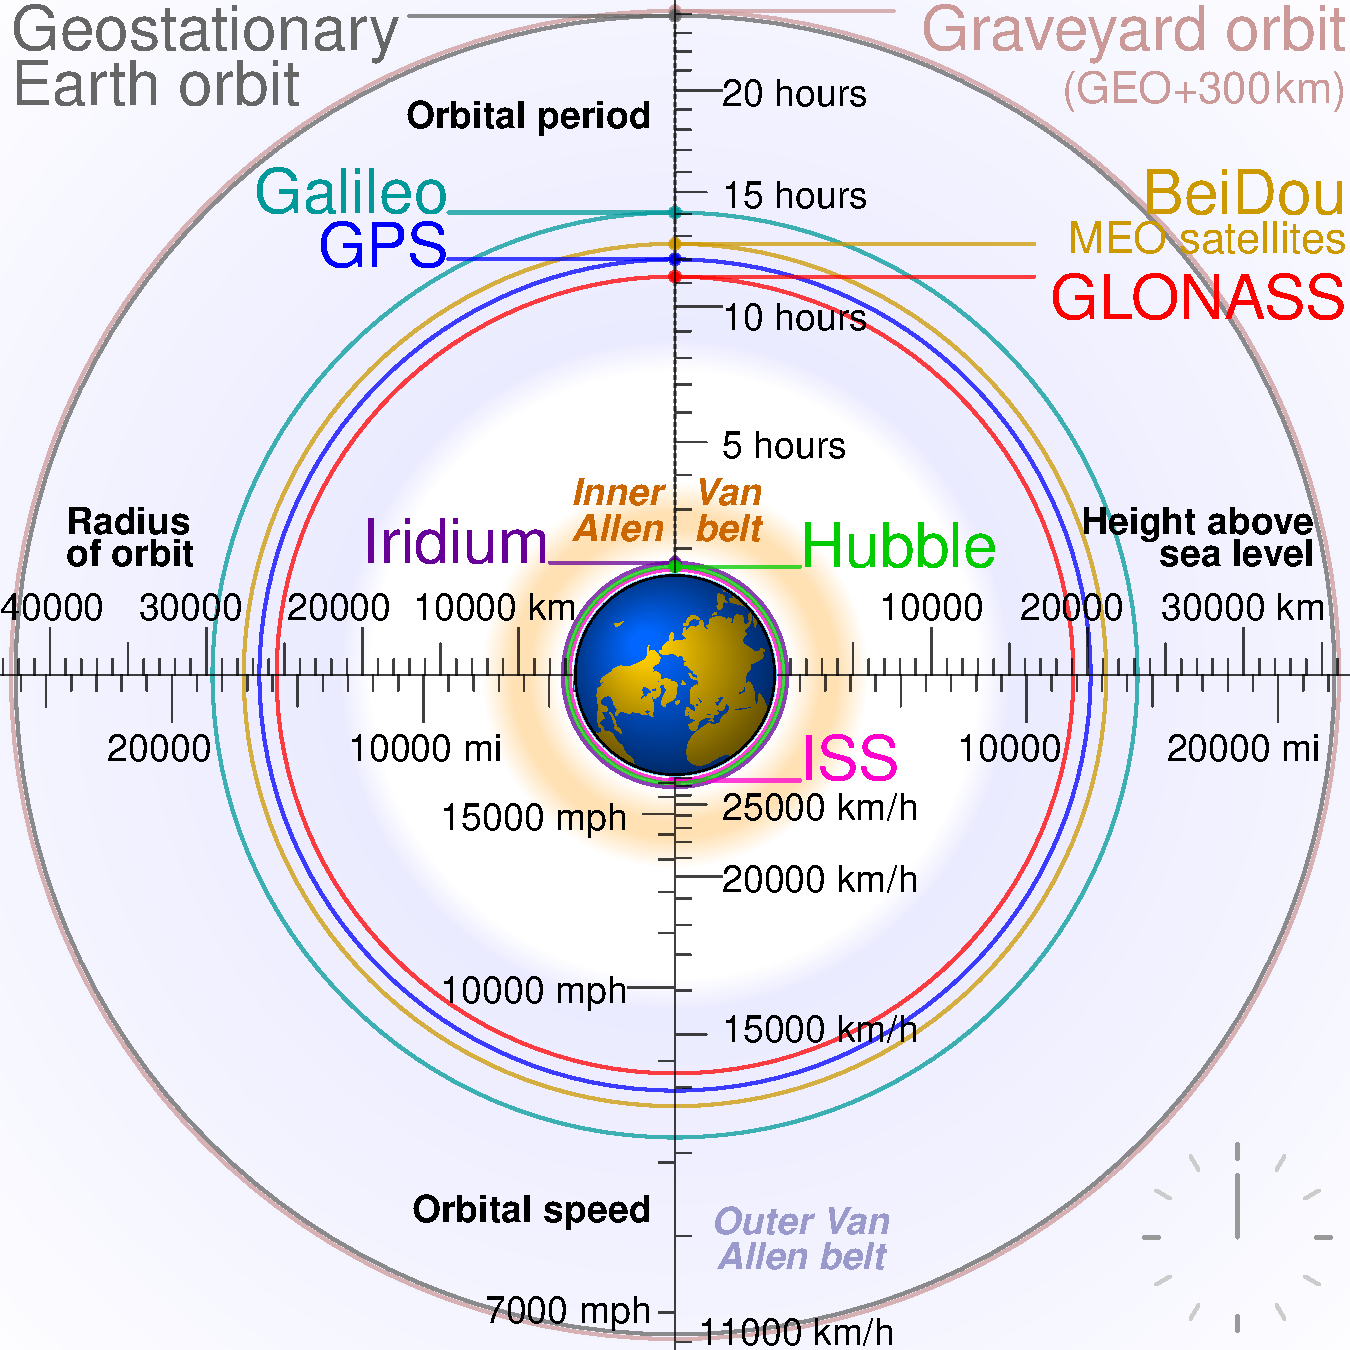
\includegraphics[width=0.19\columnwidth,valign=m]{gnss_satellite_orbits.pdf}
        }
    \end{figure}

    
    \begin{block}{Principio de Funcionamiento}
        Se toma la distancia a cuatro satélites (uno por cada incógnita: latitud, longitud, altitud y offset en tiempo del reloj del receptor) y se estima la pose por triangulación. La distancia a cada satélite se obtiene midiendo el tiempo que tarda en llegar la señal de radio del satélite.
    \end{block}
    
    \note{En el caso del GNSS estamos midiendo una señal de radio, que sabemos que viaja a la velocidad de la luz, alrededor de 300.000 km por segundo.}
    \note{La señal que recibe un receptor de GNSS no es solamente un Código Pseudo Aleatorio con fines de timing. También contiene un mensaje de navegación con información sobre la órbita exacta del satélite}
    \note{Otra manera de manejar los errores inducidos por la atmósfera es comparar la velocidad relativa de dos señales diferentes. Esta medición de doble frecuencia es muy sofisticada y solo es posible en receptores GNSS muy avanzados. Estos son los GNSS-RTK!}
    \note{Los receptores "normales" basados navegación por satélite, comparan una señal pseudoaleatoria que es enviada desde el satélite con una copia interna generada por la misma señal. Puesto que la señal del satélite tarda tiempo en alcanzar al receptor, las dos señales no se alinean correctamente, la copia del satélite se retrasa en referencia a la copia local. Al retrasar progresivamente la copia local, las dos señales se alinearán correctamente en algún momento. Este retraso es el tiempo necesario para que la señal alcance al receptor, y del resultado de esto puede ser calculada la distancia al satélite. La precisión de la medición resultante es generalmente una función de la capacidad  electrónica del receptor para comparar exactamente las dos señales.}
    
    \begin{itemize}
        \item Fuentes de ruido (Retrasos ionosféricos y atmosféricos, Efecto Multitrayectoria, Dilución de la Precisión, errores del reloj del satélite, imprecisión de órbita de los satélites)
        \item Error de posicionamiento métrico ($\sim\SI{2}{\meter}$)
    \end{itemize}
    
    \note{La Dilución de la Precisión (DOP) es una medida de la fortaleza de la geometría de los satélites y está relacionada con la distancia entre estos y su posición en el cielo. El DOP puede incrementar el efecto del error en la medición de distancia a los satélites.\\
    Un ejemplo de Dilución de la Precisión, si los satélites están en una misma línea (colineales) uno arriba del otro, queda como mal condicionado.}

\end{frame}

\begin{frame}
    \frametitle{Sistema GNSS-RTK (Real-Time Kinematics)}
    \footnotesize

    \begin{center}
        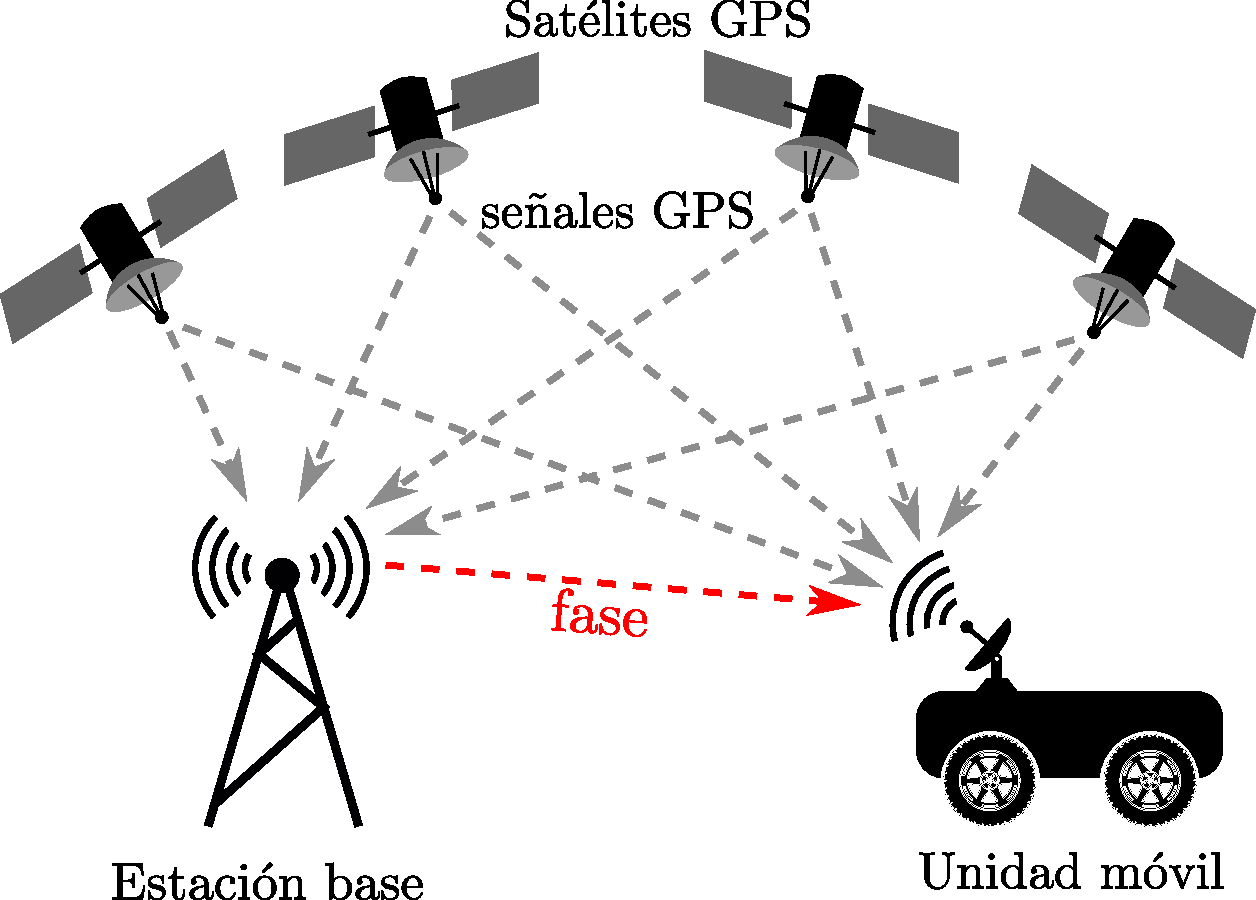
\includegraphics[width=0.3\columnwidth]{gnss_rtk_system.pdf}    
    \end{center}
    
    \only<1>{
        \begin{block}{Principio de Funcionamiento}
            \begin{itemize}
                \item Se requieren al menos dos receptores GNSS (estación base y unidad móvil). 
                \item La estación base retransmite la fase de la onda portadora de la señal enviada por el satélite \note{no tiene en cuenta los datos enviados por el satélite}
                \item La unidad móvil compara su medición de fase de la señal con la fase recibida de la estación base (\emph{Resolución de Ambig{\"u}edad})
            \end{itemize}
        \end{block}
        
        \note{ RESOLUCIÓN DE AMBIGUEDAD\\
        La sincronización entre la portadora de la señal recibida y la réplica generada en recepción permite obtener una medida de la fase de la portadora. Esta medida de fase puede ser utilizada también para estimar la distancia satélite-receptor. Sin embargo, para ello, es necesario conocer el número entero de ciclos de portadora transcurridos desde que la señal deja el satélite hasta que llega al receptor.\\
        Para realizar la sincronización entre la portadora de la señal y la réplica es necesario tener en cuenta el efecto doppler que se produce debido al movimiento relativo satélite receptor. Por ello, la frecuencia de la réplica ha de ser igual a la frecuencia de la señal transmitida con su desplazamiento doppler corregido. La sincronización se realiza mediante circuitos de enganche en fase (Phase Lock Loop, PLL) o en frecuencia (Frecuency Lock Loop, FLL). Los circuitos PLL o FLL permiten obtener medidas de fase con precisiones del orden de 0.01 ciclos de portadora.\\
        Una vez que el receptor se sincroniza con la portadora y con el código, es decir, se produce el enganche con la señal del satélite, el receptor puede medir la fase de la portadora recibida. Esta medida se obtiene de forma parecida a como se obtiene la medida de pseudodistancia, pues será el desfase que es necesario realizar a la réplica de la portadora para que se sincronice con la portadora recibida. La medida de fase se suele expresar en ciclos de portadora. Por tanto, tal como se ha descrito hasta ahora, la medida de fase será un valor decimal, no entero, indicando la fracción de ciclo de portadora transcurrido en el momento de la recepción de la señal. La distancia entre el satélite y el receptor se puede expresar en número de longitudes de onda y será igual al número entero de ciclos de portadora n transcurridos en el origen desde que la señal salió del satélite hasta que llegó al receptor, más la fracción de ciclo medida (la medida de fase). Por tanto, la medida de fase sirve como estimación de la distancia satélite-receptor pero tiene el problema de que el número entero n es desconocido. A dicho número se le denomina ambigüedad entera de ciclos de portadora. Mientras el receptor permanezca enganchado con la señal el número entero n desconocido permanecerá constante, pues el receptor registra la variación del número entero de ciclos en las propias medidas de fase. La figura 1.7 ilustra esta circunstancia. En el instante t 0 se produce el enganche, obteniéndose la medida phi 0 y siendo desconocido el número de ciclos n. A partir de entonces, el receptor registra la variación de ciclos que se van produciendo y en los instantes sucesivos las medidas de fase phi i estarán formadas por una parte fraccional y una parte entera: la diferencia entre el número de ciclos transcurridos y el número n de la medida inicial. Por tanto, el único valor desconocido es el número entero de ciclos n inicial.}
   }
    \only<2>{ 
        \begin{itemize}
            \item Error de posicionamiento submétrico ($\sim\SI{0.05}{\meter}$).
            \item Alcance de \SI{10}{\km}
            \item GNSS-RTK es una evolución de DGNSS (Differential-GNSS). GNSS-RTK utiliza un nuevo protocolo de comunicación (RTCM3) y un mejor algoritmo de corrección.
            \item NTRIP (\emph{Networked Transport of RTCM via Internet Protocol}) correcciones por internet desde una estación permanente
        \end{itemize}
        \note{DGNSS vs GNSS-RTK: https://youtu.be/SOYDTxbX4mM?si=NmRR0_DU11HEORfo}
    }
\end{frame}

\begin{frame}
    \frametitle{Estación Permamente GPS}
    \begin{center}
        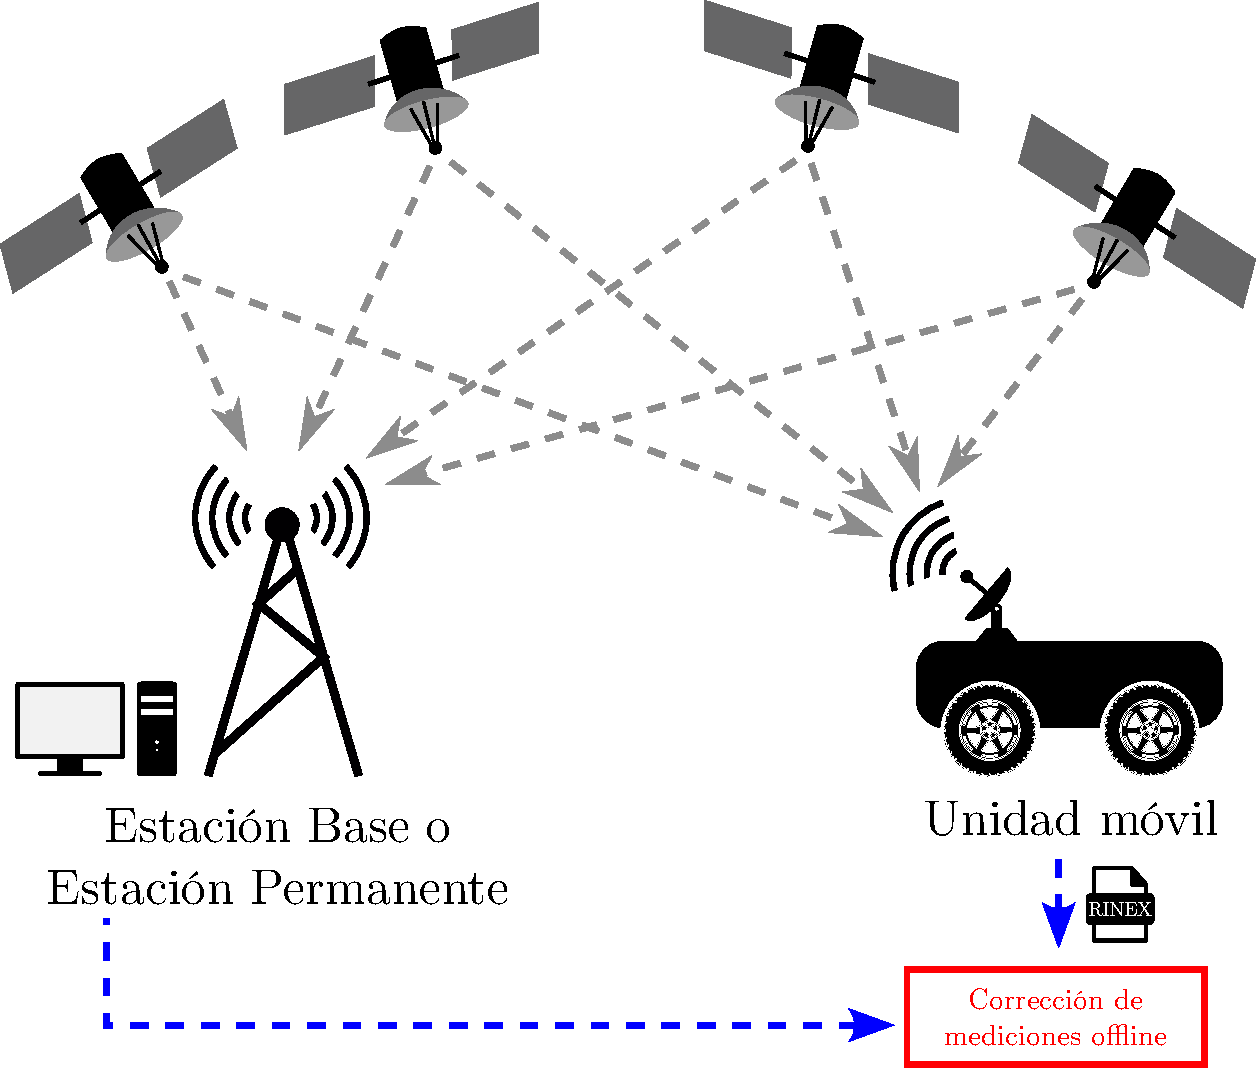
\includegraphics[width=0.3\columnwidth]{gnss_ppk_system.pdf}
    \end{center}

    \href{https://www.fceia.unr.edu.ar/gps/}{https://www.fceia.unr.edu.ar/gps/}

    RINEX (\emph{Receiver Independent Exchange Format})  permite posprocesar los datos recibidos para producir un resultado más preciso, generalmente con otros datos desconocidos para el receptor original, como mejores modelos de las condiciones atmosféricas en el momento de la medición.
    RINEX es el formato estándar que permite la gestión y disposición de las medidas generadas por un receptor, así como su tratamiento off-line por multitud de aplicaciones, sea cual sea el fabricante tanto del receptor como de la aplicación informática.

\end{frame}


\begin{frame}
    \frametitle{Sistema GNSS-PPK (Post Processed Kinematic)}
    \begin{center}
        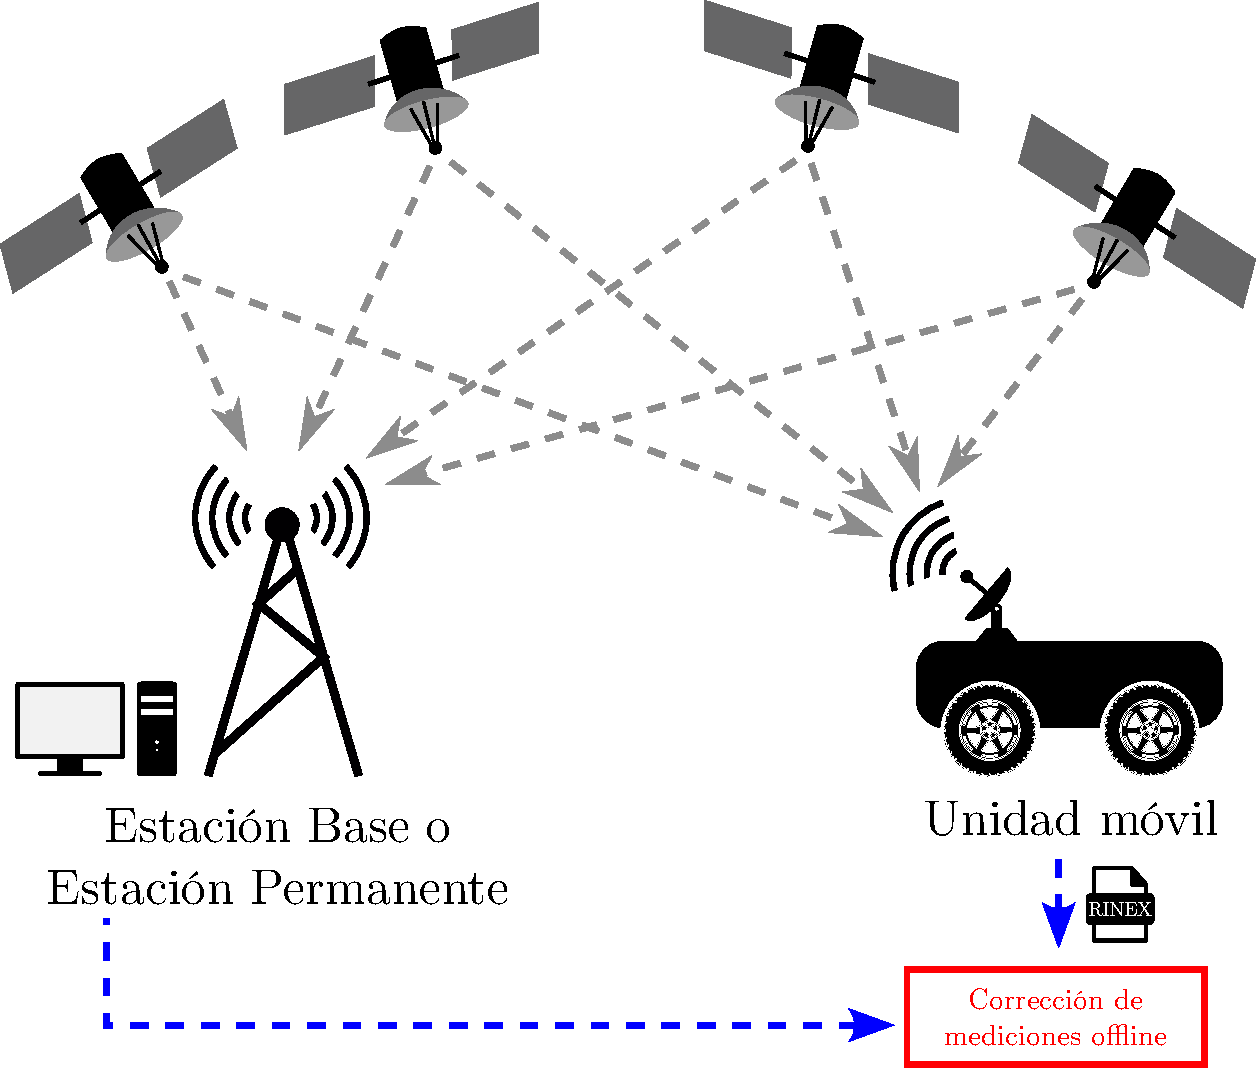
\includegraphics[width=0.3\columnwidth]{gnss_ppk_system.pdf}
    \end{center}

    El PPK (Post Processed Kinematic), a diferencia del RTK, realiza un proceso de datos a posteriori (offline).
    En la imagen vemos que, tanto la base como el drone, reciben lecturas de las diferentes constelaciones de satélites. Pero, a diferencia del RTK, no hay un enlace de datos constante entre el drone y la base, ya que ambos registran en una memoria esa información que después del vuelo deberemos descargar, normalmente en archivos con formato RINEX, para postprocesar y obtener nuestra solución.
    
\end{frame}

\begin{frame}
    \frametitle{Sistema GNSS-PPP (Precise Point Positioning)}
    \begin{center}
        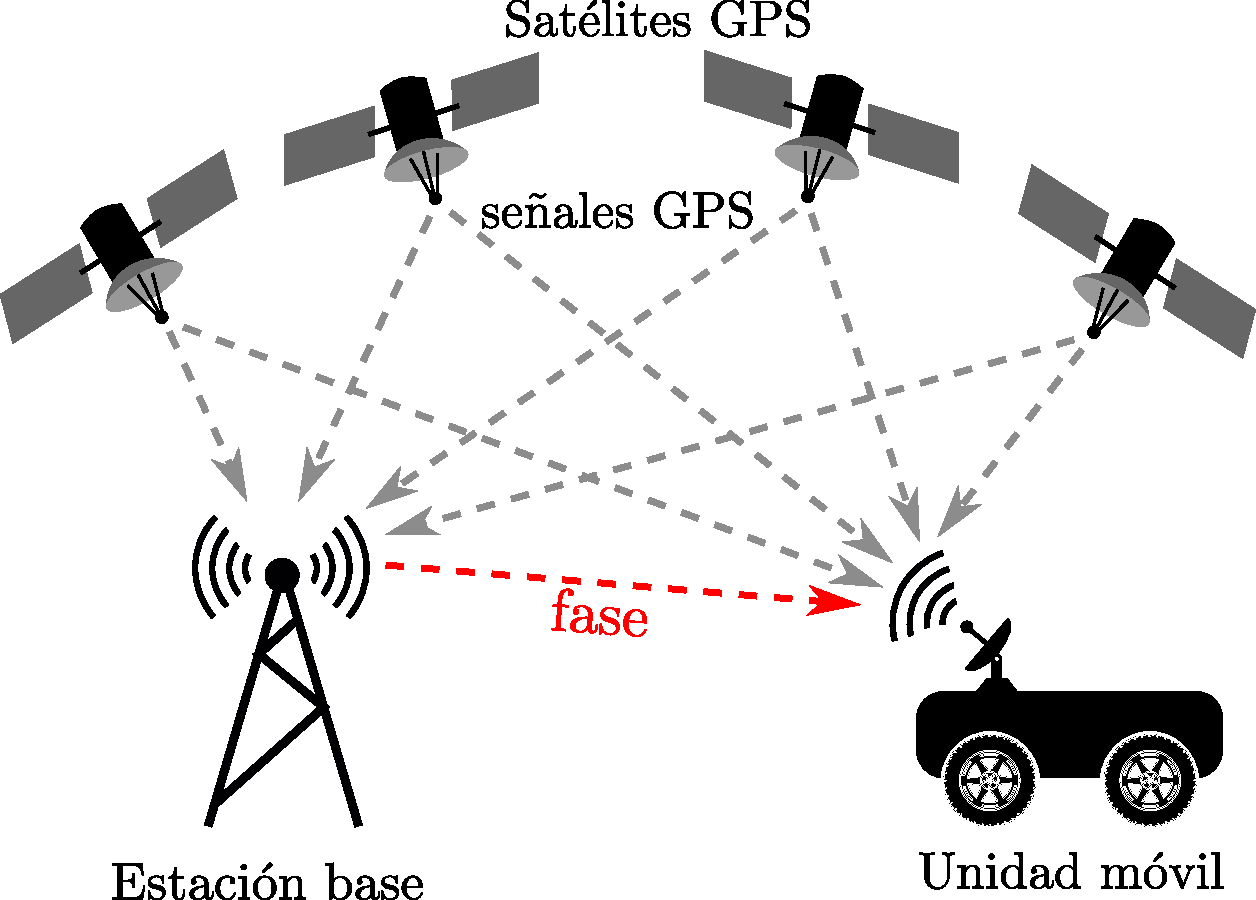
\includegraphics[width=0.3\columnwidth]{gnss_rtk_system.pdf}
    \end{center}

\end{frame}

\begin{frame}
    \frametitle{NTRIP}
    \begin{center}
        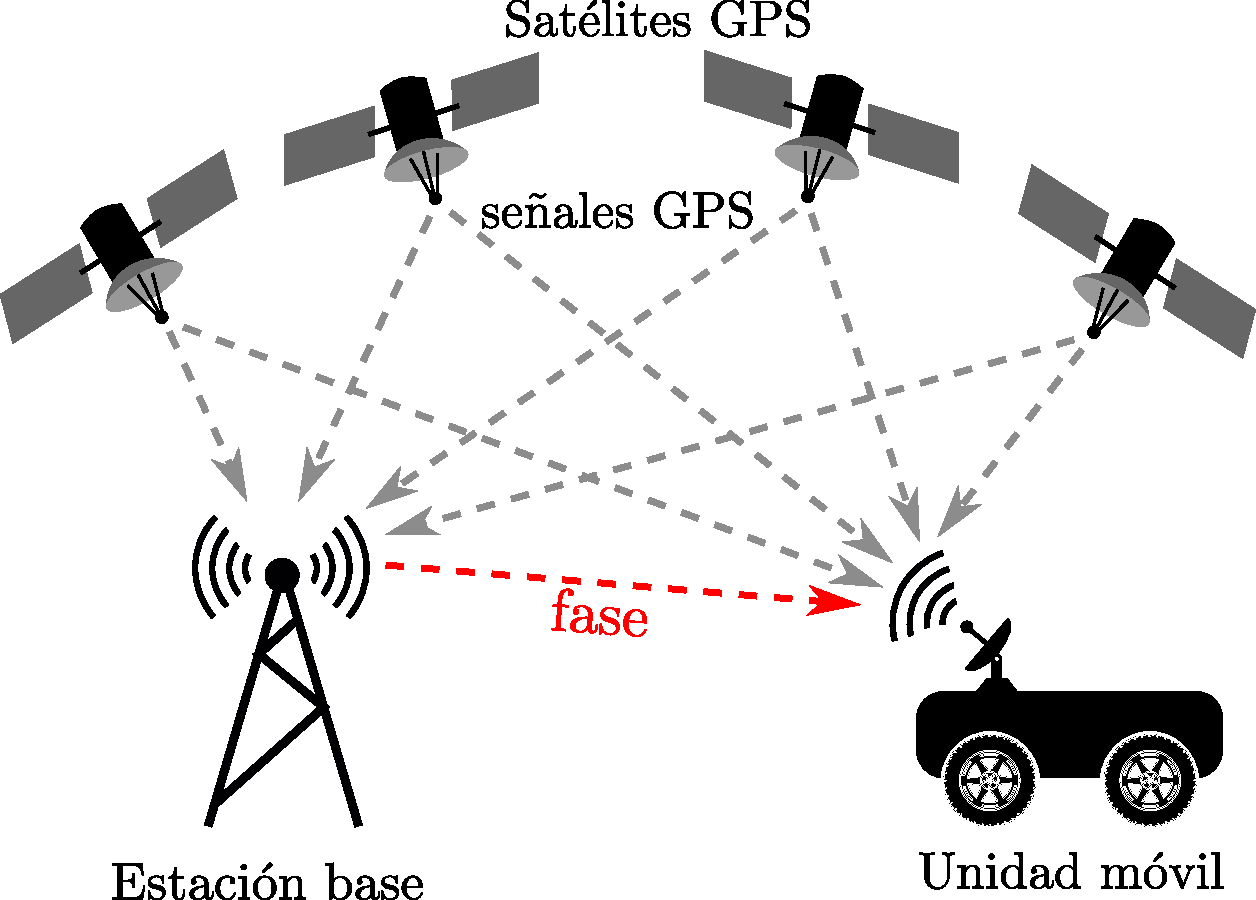
\includegraphics[width=0.3\columnwidth]{gnss_rtk_system.pdf}
    \end{center}

\end{frame}

\begin{frame}
    \frametitle{Sistema GPS-RTK características}
    \begin{itemize}
        \item Al menos dos receptores GPS (estación base y unidad móvil)
        \item La estación base retransmite la fase de la onda portadora de la señal enviada por el satelite \note{no tiene en cuenta los datos enviados por el satelite}
        \item La unidad móvil compara su medición de fase de la señal con la fase recibida de la estación base (\emph{Resolución de Ambig\"uedad})
        \item Error de posicionamiento submétrico.
        \item Alcance de \SI{10}{\km}
    \end{itemize}
    \centering
    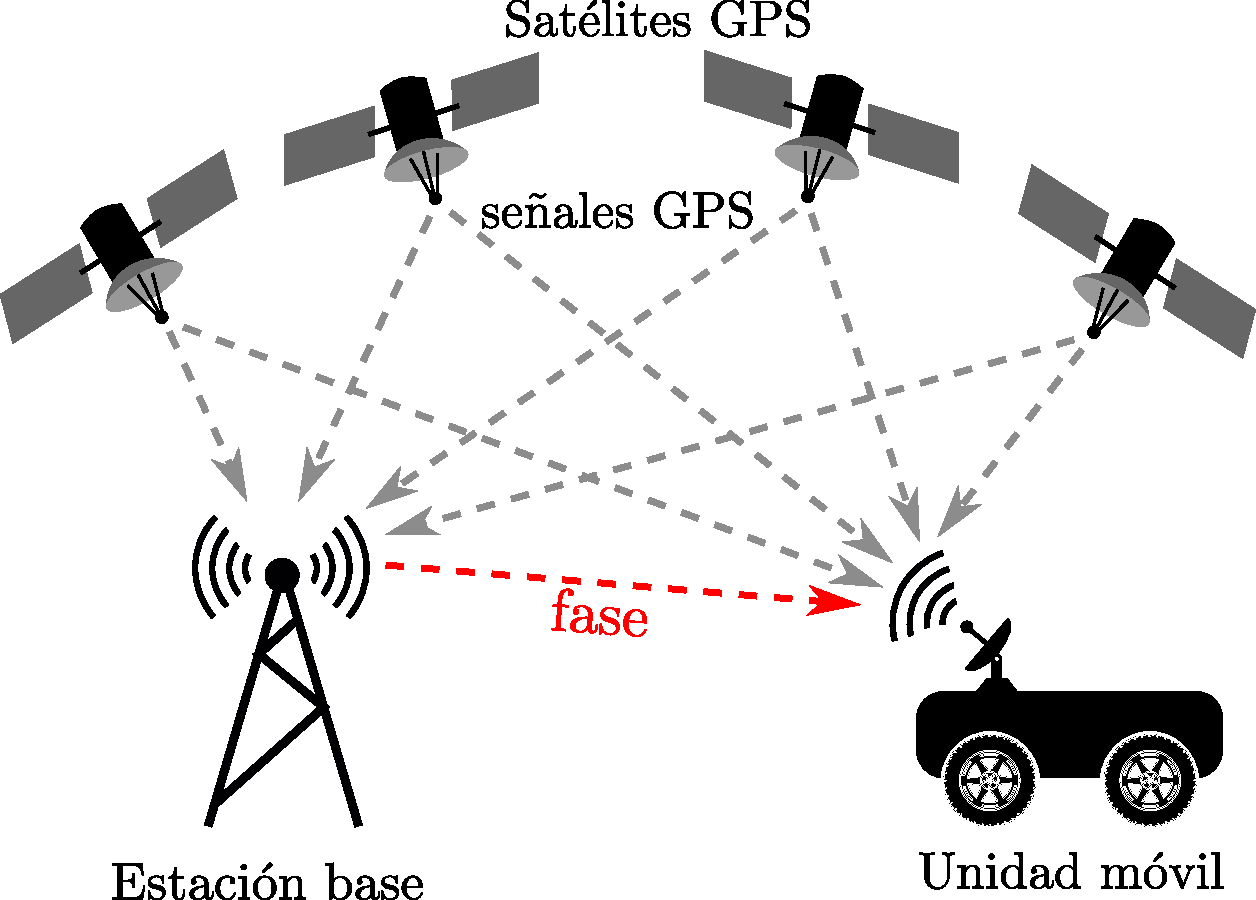
\includegraphics[width=0.5\columnwidth]{gps_rtk_system.pdf}
    %
    \note{ RESOLUCIÓN DE AMBIGUEDAD\\
        La sincronización entre la portadora de la señal recibida y la réplica generada en recepción permite obtener una medida de la fase de la portadora. Esta medida de fase puede ser utilizada también para estimar la distancia satélite-receptor. Sin embargo, para ello, es necesario conocer el número entero de ciclos de portadora transcurridos desde que la señal deja el satélite hasta que llega al receptor.\\
        Para realizar la sincronización entre la portadora de la señal y la réplica es necesario tener en cuenta el efecto doppler que se produce debido al movimiento relativo satélite receptor. Por ello, la frecuencia de la réplica ha de ser igual a la frecuencia de la señal transmitida con su desplazamiento doppler corregido. La sincronización se realiza mediante circuitos de enganche en fase (Phase Lock Loop, PLL) o en frecuencia (Frecuency Lock Loop, FLL). Los circuitos PLL o FLL permiten obtener medidas de fase con precisiones del orden de 0.01 ciclos de portadora.\\
        Una vez que el receptor se sincroniza con la portadora y con el código, es decir, se produce el enganche con la señal del satélite, el receptor puede medir la fase de la portadora recibida. Esta medida se obtiene de forma parecida a como se obtiene la medida de pseudodistancia, pues será el desfase que es necesario realizar a la réplica de la portadora para que se sincronice con la portadora recibida. La medida de fase se suele expresar en ciclos de portadora. Por tanto, tal como se ha descrito hasta ahora, la medida de fase será un valor decimal, no entero, indicando la fracción de ciclo de portadora transcurrido en el momento de la recepción de la señal. La distancia entre el satélite y el receptor se puede expresar en número de longitudes de onda y será igual al número entero de ciclos de portadora n transcurridos en el origen desde que la señal salió del satélite hasta que llegó al receptor, más la fracción de ciclo medida (la medida de fase). Por tanto, la medida de fase sirve como estimación de la distancia satélite-receptor pero tiene el problema de que el número entero n es desconocido. A dicho número se le denomina ambigüedad entera de ciclos de portadora. Mientras el receptor permanezca enganchado con la señal el número entero n desconocido permanecerá constante, pues el receptor registra la variación del número entero de ciclos en las propias medidas de fase. La figura 1.7 ilustra esta circunstancia. En el instante t 0 se produce el enganche, obteniéndose la medida phi 0 y siendo desconocido el número de ciclos n. A partir de entonces, el receptor registra la variación de ciclos que se van produciendo y en los instantes sucesivos las medidas de fase phi i estarán formadas por una parte fraccional y una parte entera: la diferencia entre el número de ciclos transcurridos y el número n de la medida inicial. Por tanto, el único valor desconocido es el número entero de ciclos n inicial.}
\end{frame}


\begin{frame}
    \frametitle{Cámara basada en eventos}
    
    
    \TODO{Event based camera video}
    
    \begin{figure}[!h]
        \centering
        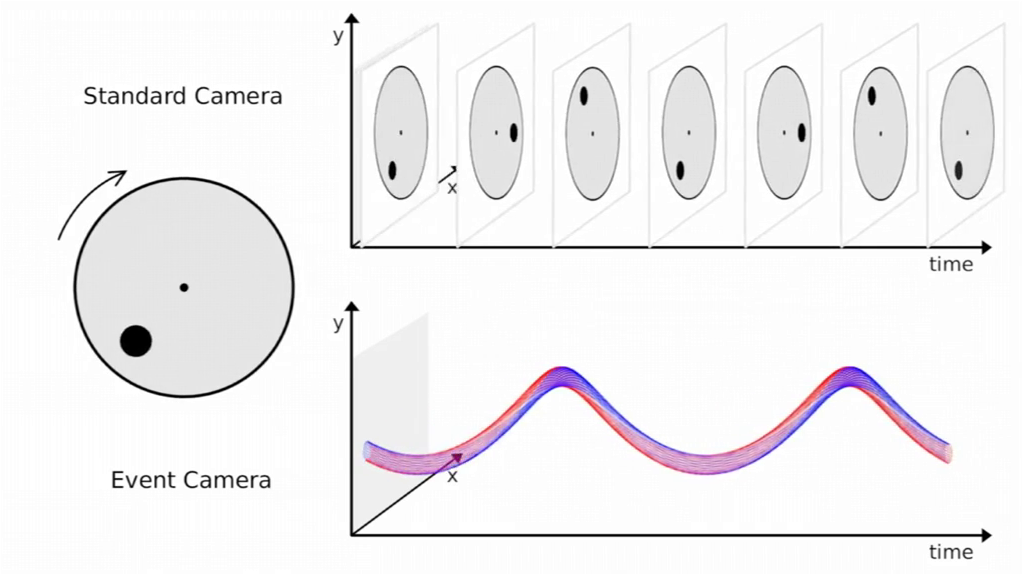
\includegraphics[width=0.8\columnwidth]{images/event_camera.png}
    \end{figure}

\end{frame}

\section{Bibliografía}
\begin{frame}
	\frametitle{Bibliografía}
	
	Capítulo 3 y 7 de: \cite{thrun2005probabilistic}
	
	Shon and Lindsen: Manipulating the Multivariate Gaussian Density
	
	\printbibliography
	
\end{frame}

\end{document}
